\chapter{Results Discussion}
\label{cha:results_discussion}

In this chapter, we analyze the results of our experiments, focusing on how the
agent performs in different maps and goals configuration to evaluate the agent's
ability to navigate the map and successfully complete its tasks. We examine how the
placement of goal tiles affects decision-making, assess whether the model
struggles with retrieving relevant information, and compare the performance in the
same slice of different maps.

Our primary objective is to evaluate the agent's ability to navigate the map and
successfully complete pickup and delivery tasks.

In tasks where the agent's goal is to pick up a parcel, the target tile
corresponds to the one containing the parcel. Conversely, in delivery tasks, the
goal tile is the specific location where the agent must deliver the parcel.

The placement of goal tiles within the game map was carefully designed to ensure
consistency and meaningful evaluation across both pickup and delivery tasks.
Specifically, we aimed to use the same goal tiles for both objectives, allowing
for direct comparisons between the two. In the pickup scenario, the goal is
always explicitly stated at the end of the prompt, making it immediately available
to the LLM. However, in the delivery scenario, the agent must retrieve the
delivery location from the provided map description, requiring it to process and
extract the relevant information effectively.

To evaluate how well the model handles goal retrieval, we selected three
distinct goal positions: the top-right, center, and bottom-right cells of the map.
These placements ensure that the goal appears in different parts of the map
description inside the prompt, allowing us to assess whether the ``needle in a haystack"
problem, as discussed in related literature, affects the model's ability to
locate and act on relevant information during the delivery task.

In the final section, we will discuss the different LLMs used in the agent's decision-making
process. As a general observation, GPT-3.5 performed worse compared to the more advanced
GPT-4o variants. Among the newer models, GPT-4o and GPT-4o-mini demonstrated similar
performance, with both outperforming GPT-3.5. Due to budget constraints, the
majority of our analysis was conducted using GPT-4o-mini, as it provides a cost-effective
yet high-quality alternative. However, our qualitative findings can be reasonably
extended to GPT-4o as well, given their comparable performance, and to all models
with similar performance and/or architecture. Each LLM call had an average input
size of approximately 250 tokens, with only a single token as output. The cost
per call was approximately \$0.000038.

\section{Map Orientation}

In this section, we analyze the impact of map orientation on the agent's decision-making
process. Since the prompt did not explicitly reference any specific orientation,
the model had to infer it based solely on the provided map description and its training
data. By examining the model's outputs, we can determine its perceived orientation
of the map and assess whether any biases emerge.

To investigate this, we analyzed the data using two different origin conventions.
The raw data was structured with the $(0,0)$ coordinate in the top-left corner,
but we also transformed the map to simulate a bottom-left origin by adjusting
all coordinates accordingly. We then ran the agent in both configurations—one using
the original top-left origin and another using the simulated bottom-left origin—to
compare how the agent's actions varied under different map orientations.

As illustrated in Figure \ref{fig:orientation}, the heatmaps of the agent's
actions appear nearly identical, except for a 90-degree rotation. The small
differences between the two cases can be attributed to the way the data was
structured in the prompt, which may have influenced the model's text generation.

\begin{figure}[h]
  \centering
  \begin{minipage}[b]{0.45\textwidth}
    \centering
    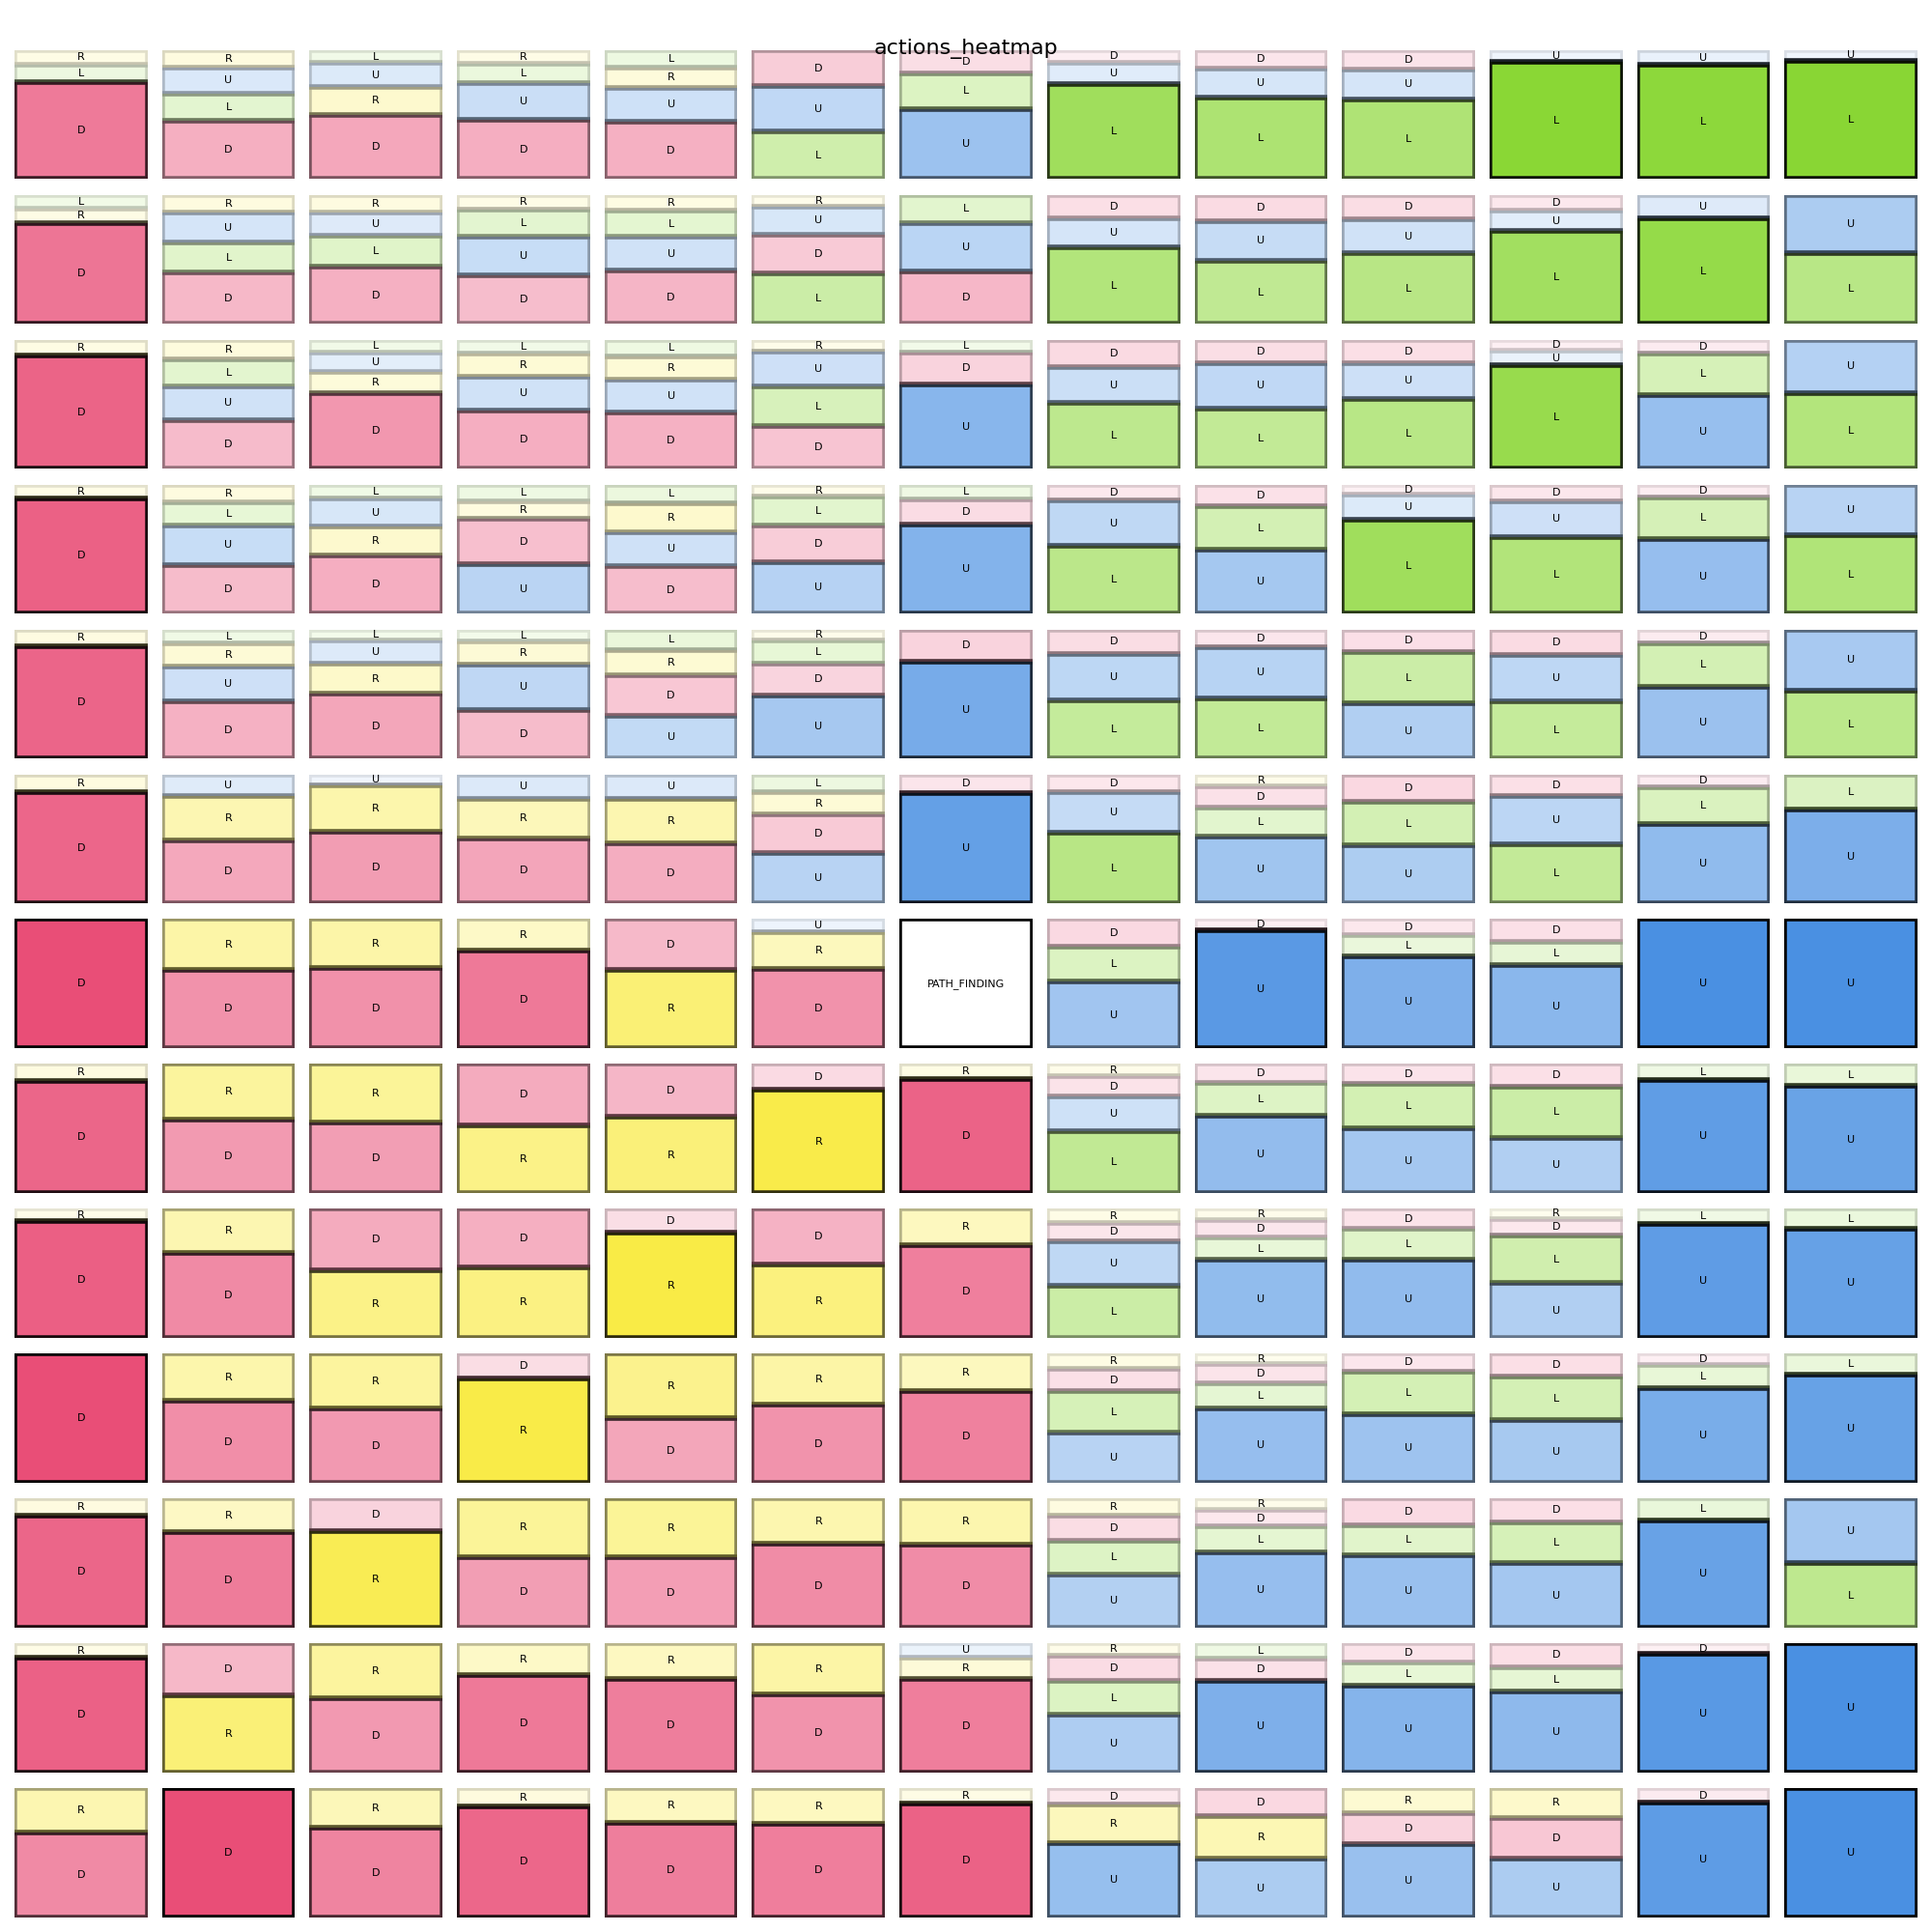
\includegraphics[width=\textwidth]{
      images/results_discussion/actions_heatmapBL.png
    }
    \caption{Bottom Left Origin Orientation}
    \label{fig:heatmapBL}
  \end{minipage}
  \hfill
  \begin{minipage}[b]{0.45\textwidth}
    \centering
    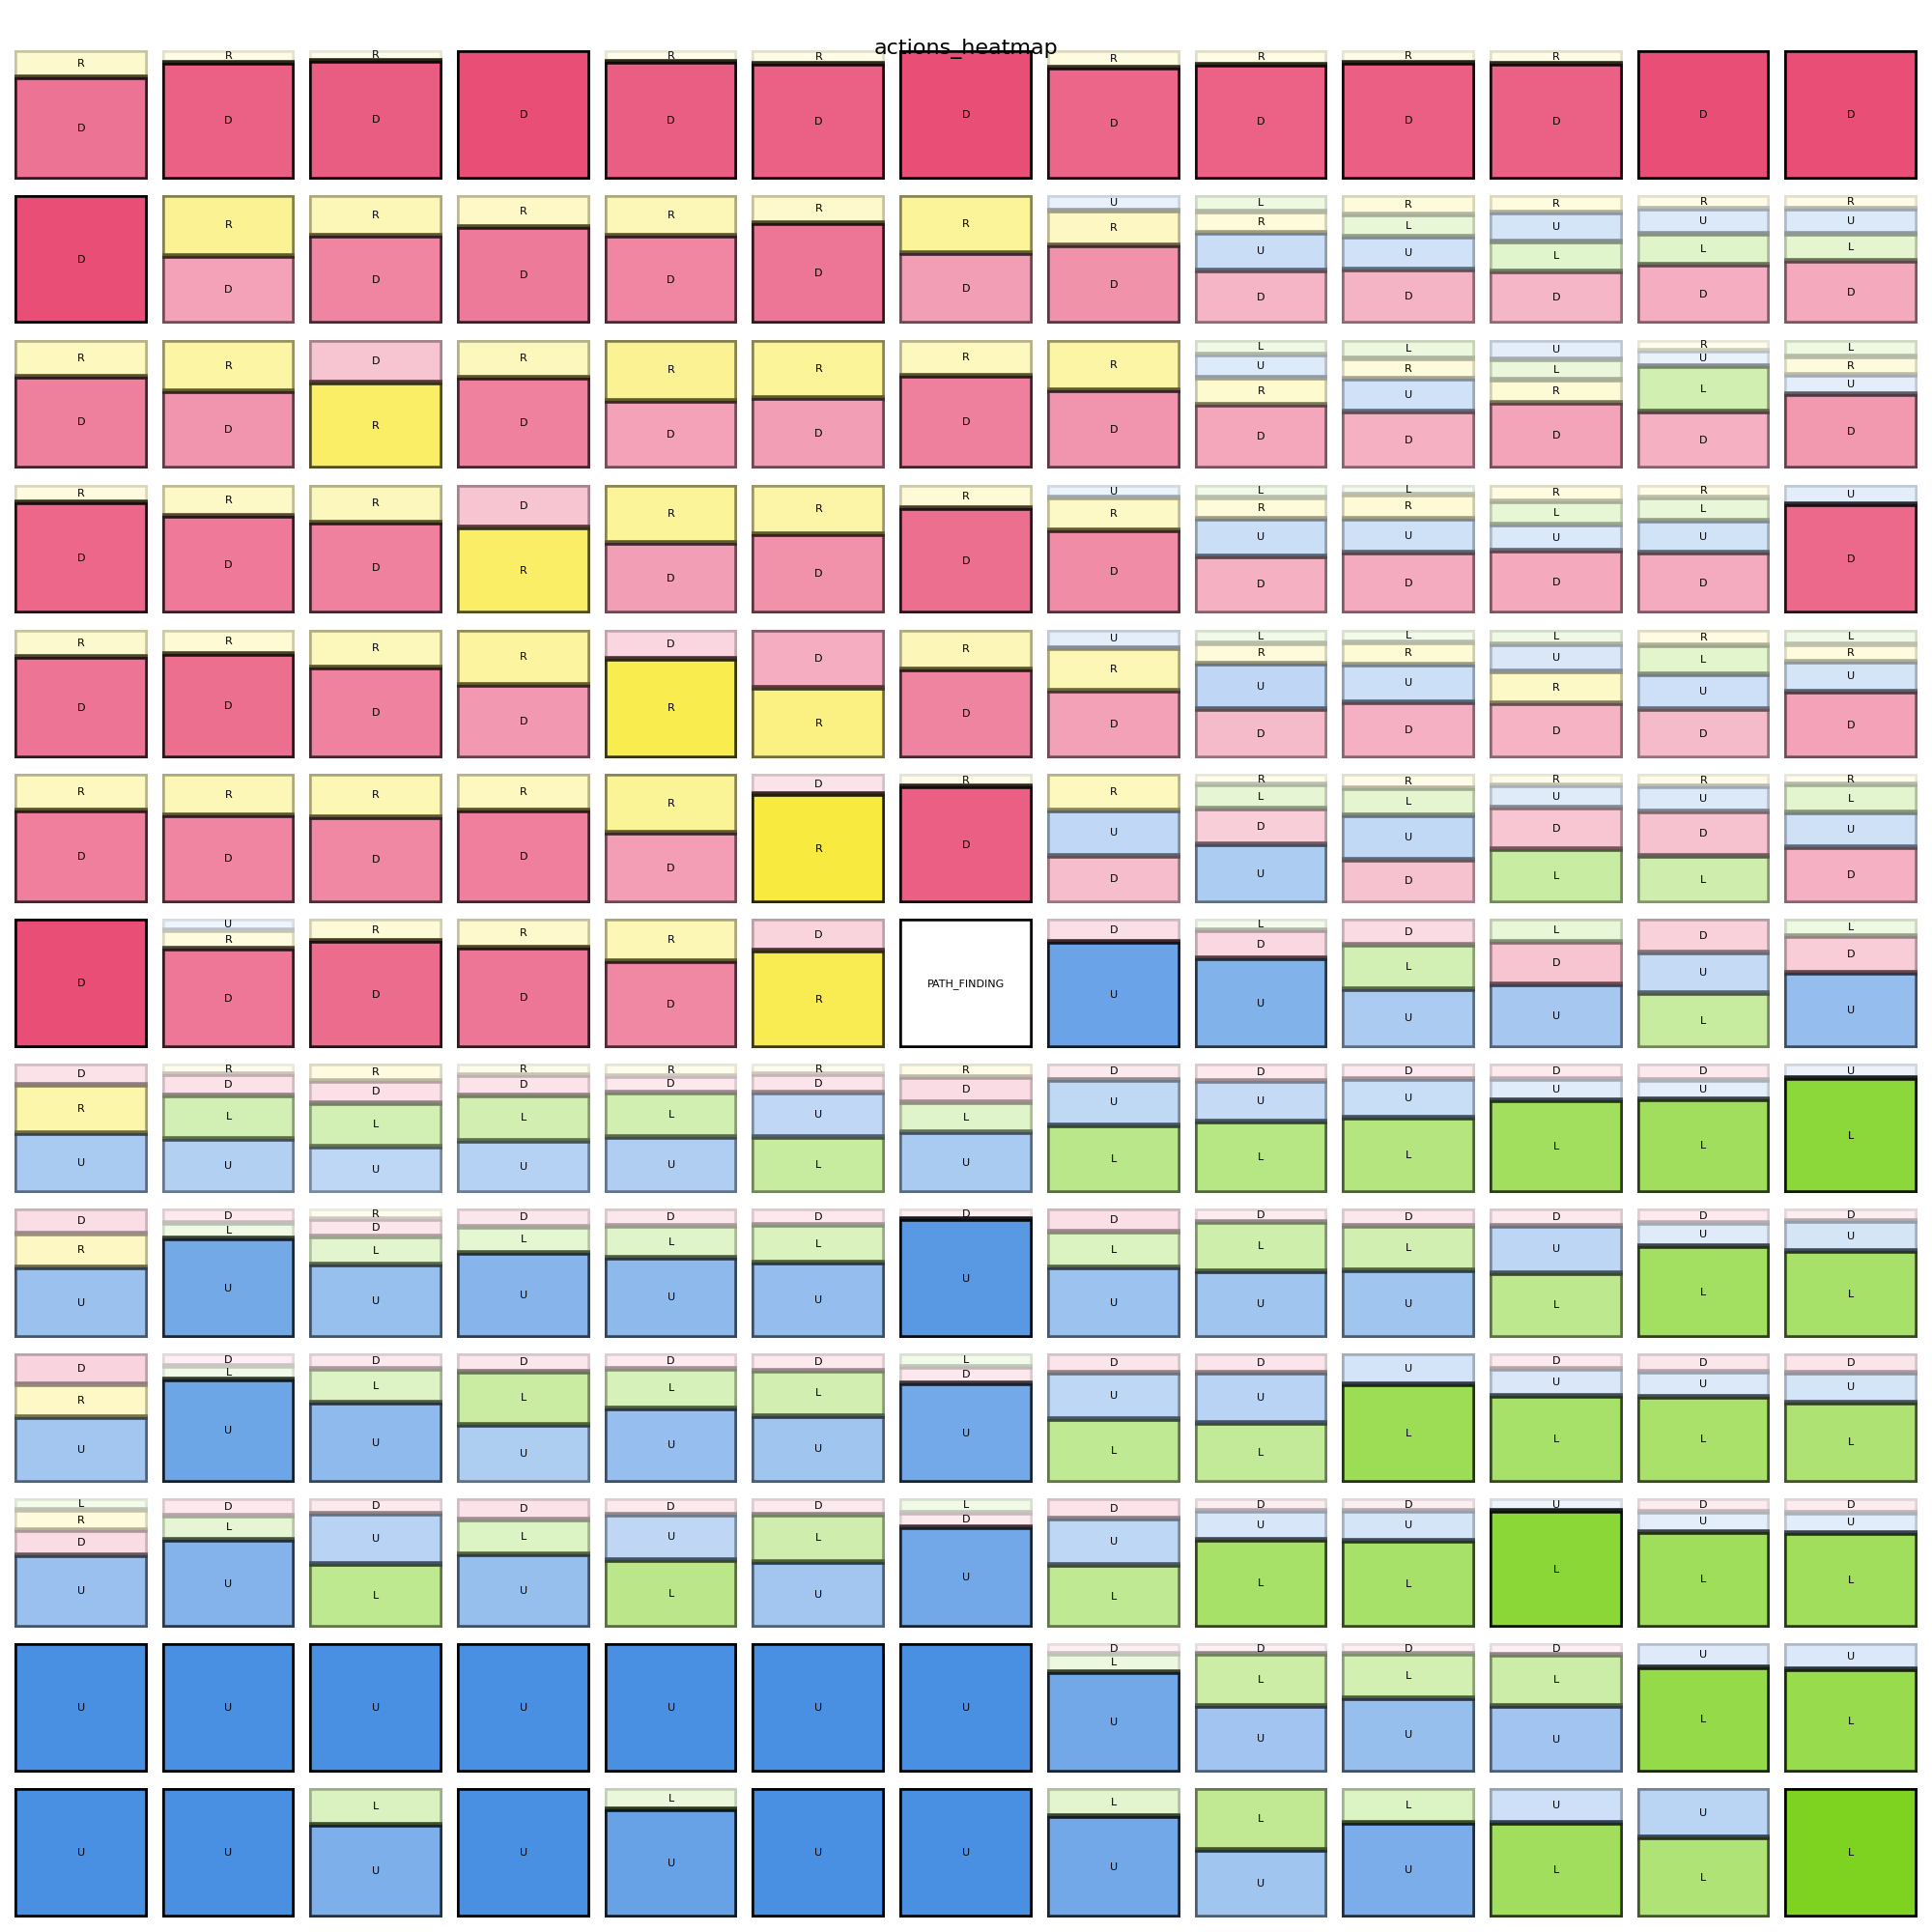
\includegraphics[width=\textwidth]{
      images/results_discussion/actions_heatmapTL.png
    }
    \caption{Top Left Origin Orientation}
    \label{fig:heatmapTL}
  \end{minipage}
  \caption{Heatmaps showing actions' probability with different map orientations}
  \label{fig:orientation}
\end{figure}

To further analyze the effect of orientation, we examined the correctness heatmaps
for both configurations, as shown in Figure \ref{fig:orientation_correctness}. The
results reveal a clear bias toward the top-left origin orientation, which we
refer to as the "programming origin," in contrast to the "Cartesian origin" commonly
used in mathematical contexts.

This bias may stem from the way the map was presented to the model. In our
specific implementation, the map was formatted as a list of tiles extracted from
a minimally edited JSON file. Given that JSON and other common data structures
in computer science often follow a top-left origin convention, it is likely that
the LLM was implicitly influenced by its prior knowledge from programming-related
contexts.

\vspace{5mm}
\begin{figure}[h]
  \centering
  \begin{minipage}[b]{0.45\textwidth}
    \centering
    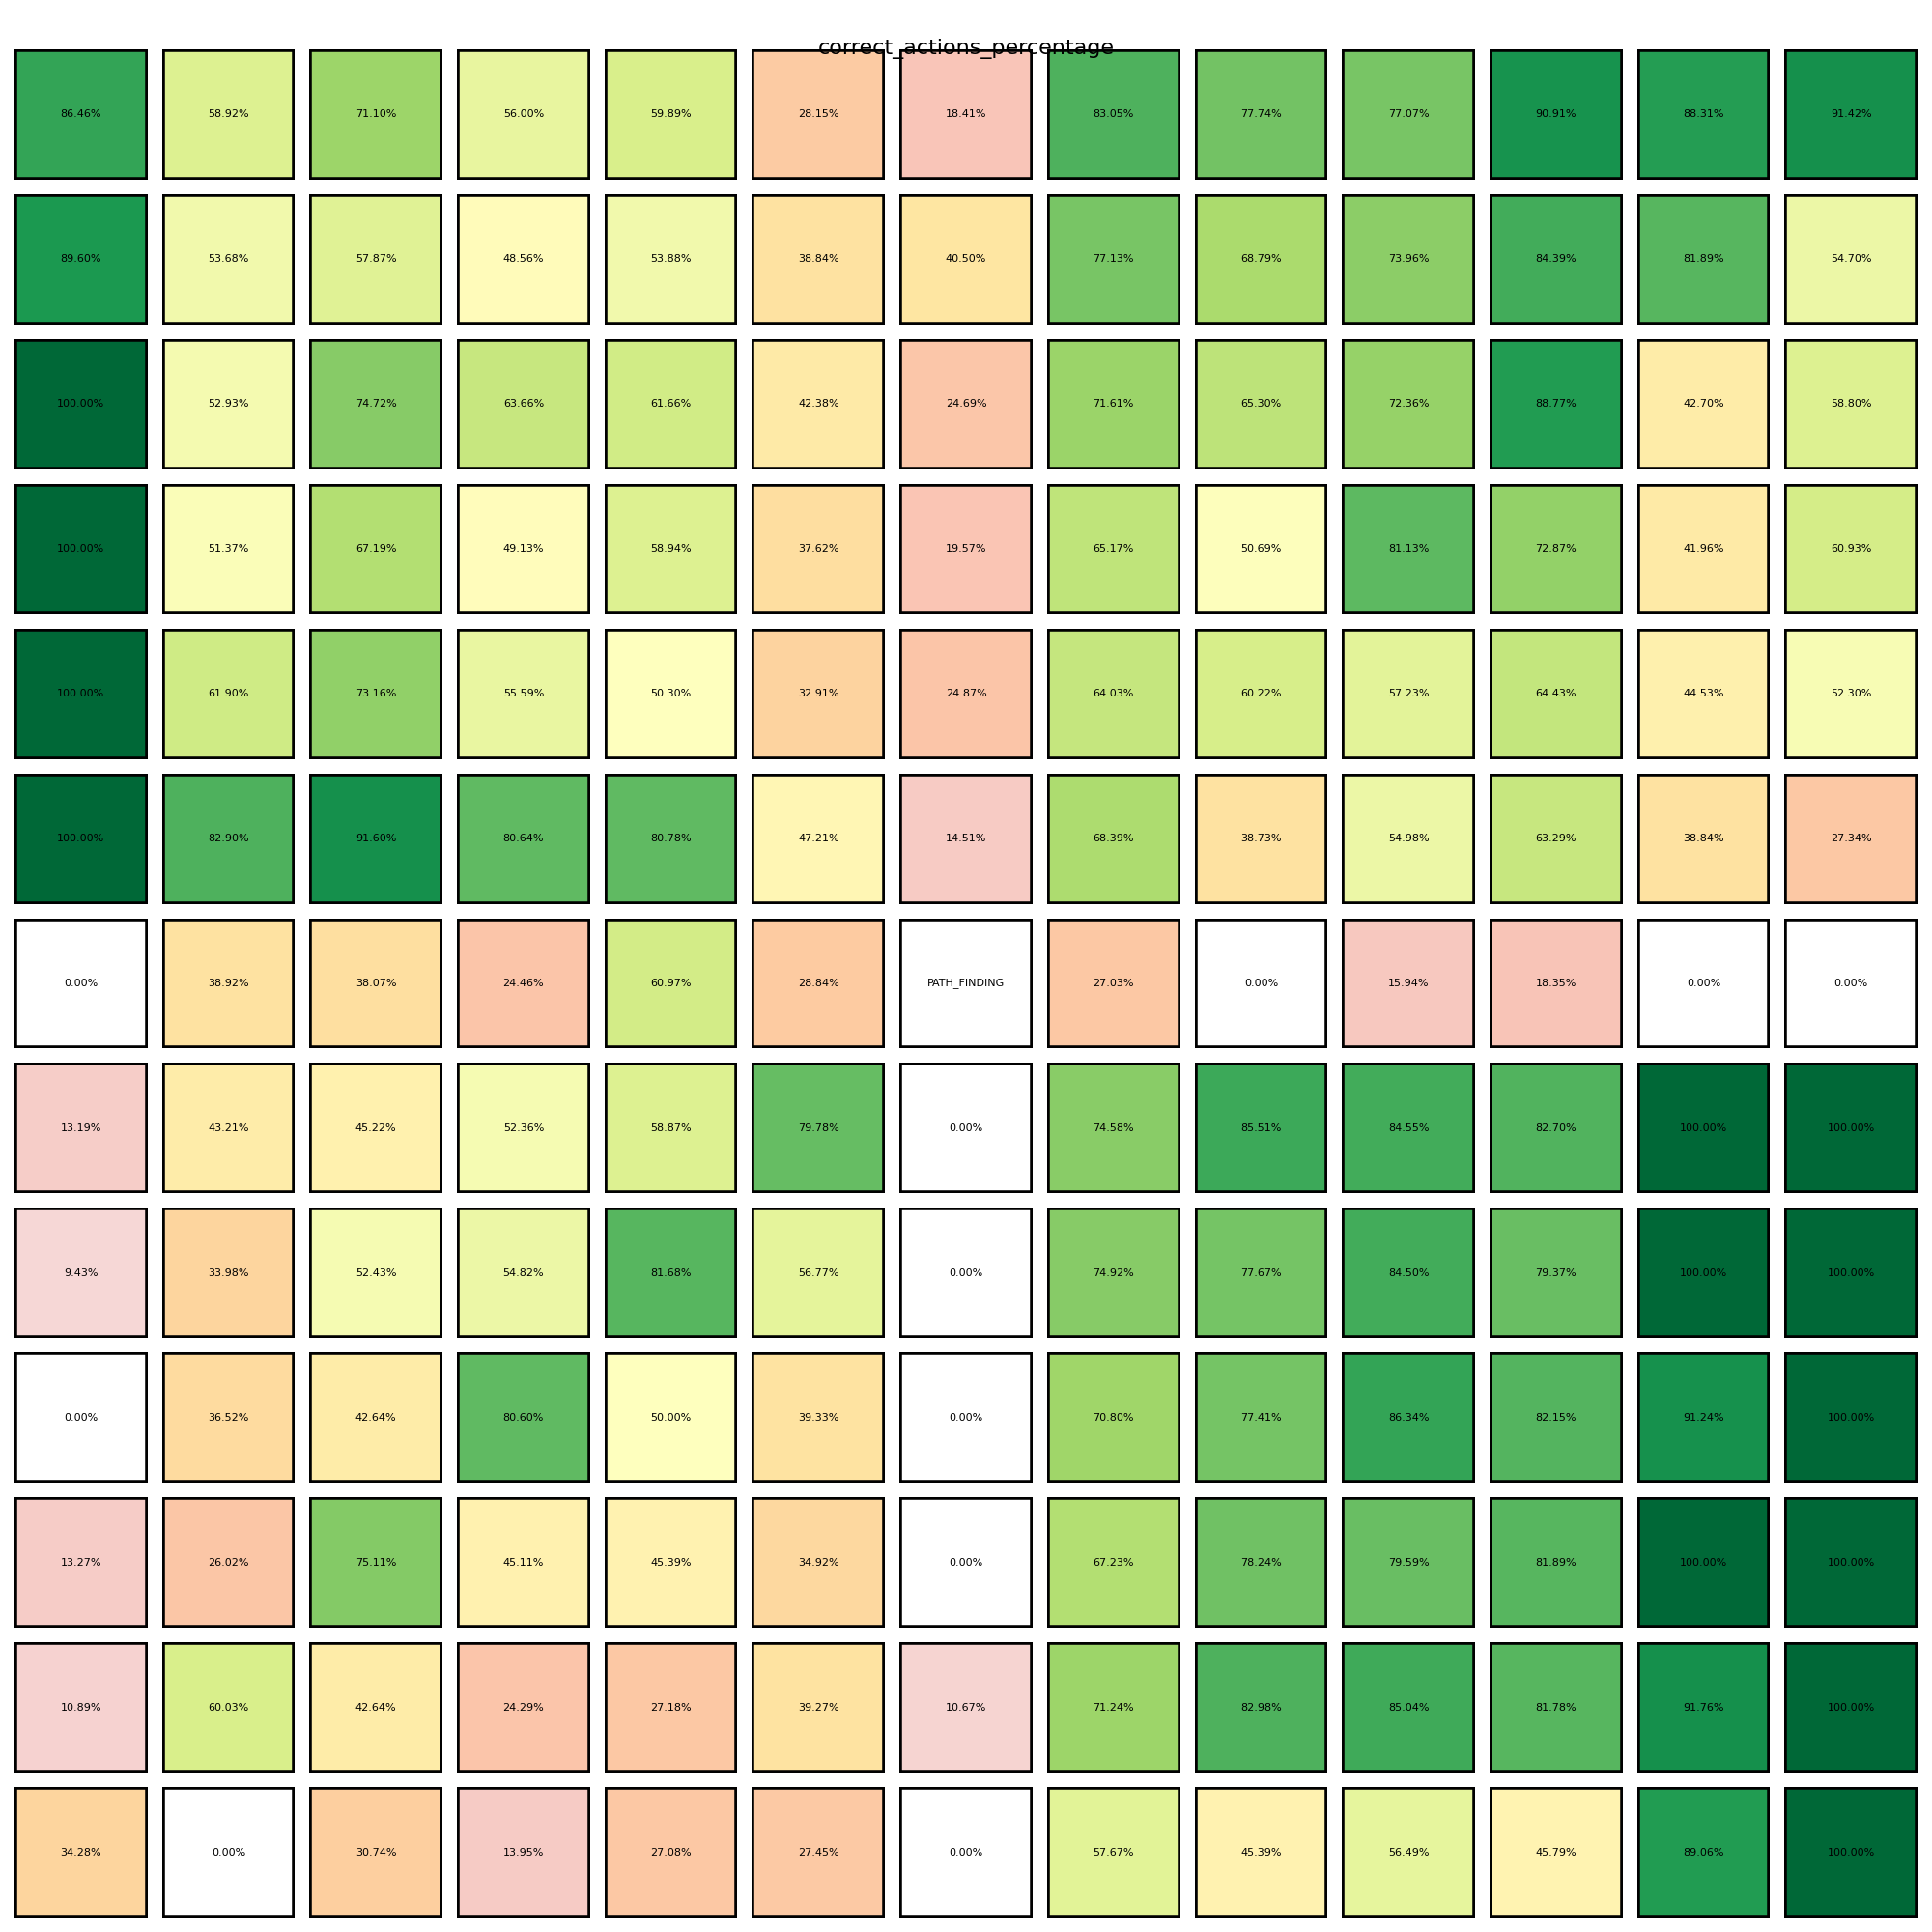
\includegraphics[width=\textwidth]{
      images/results_discussion/correctness_hm_BL.png
    }
    \caption{Bottom Left Origin Orientation}
    \label{fig:heatmapBL}
  \end{minipage}
  \hfill
  \begin{minipage}[b]{0.45\textwidth}
    \centering
    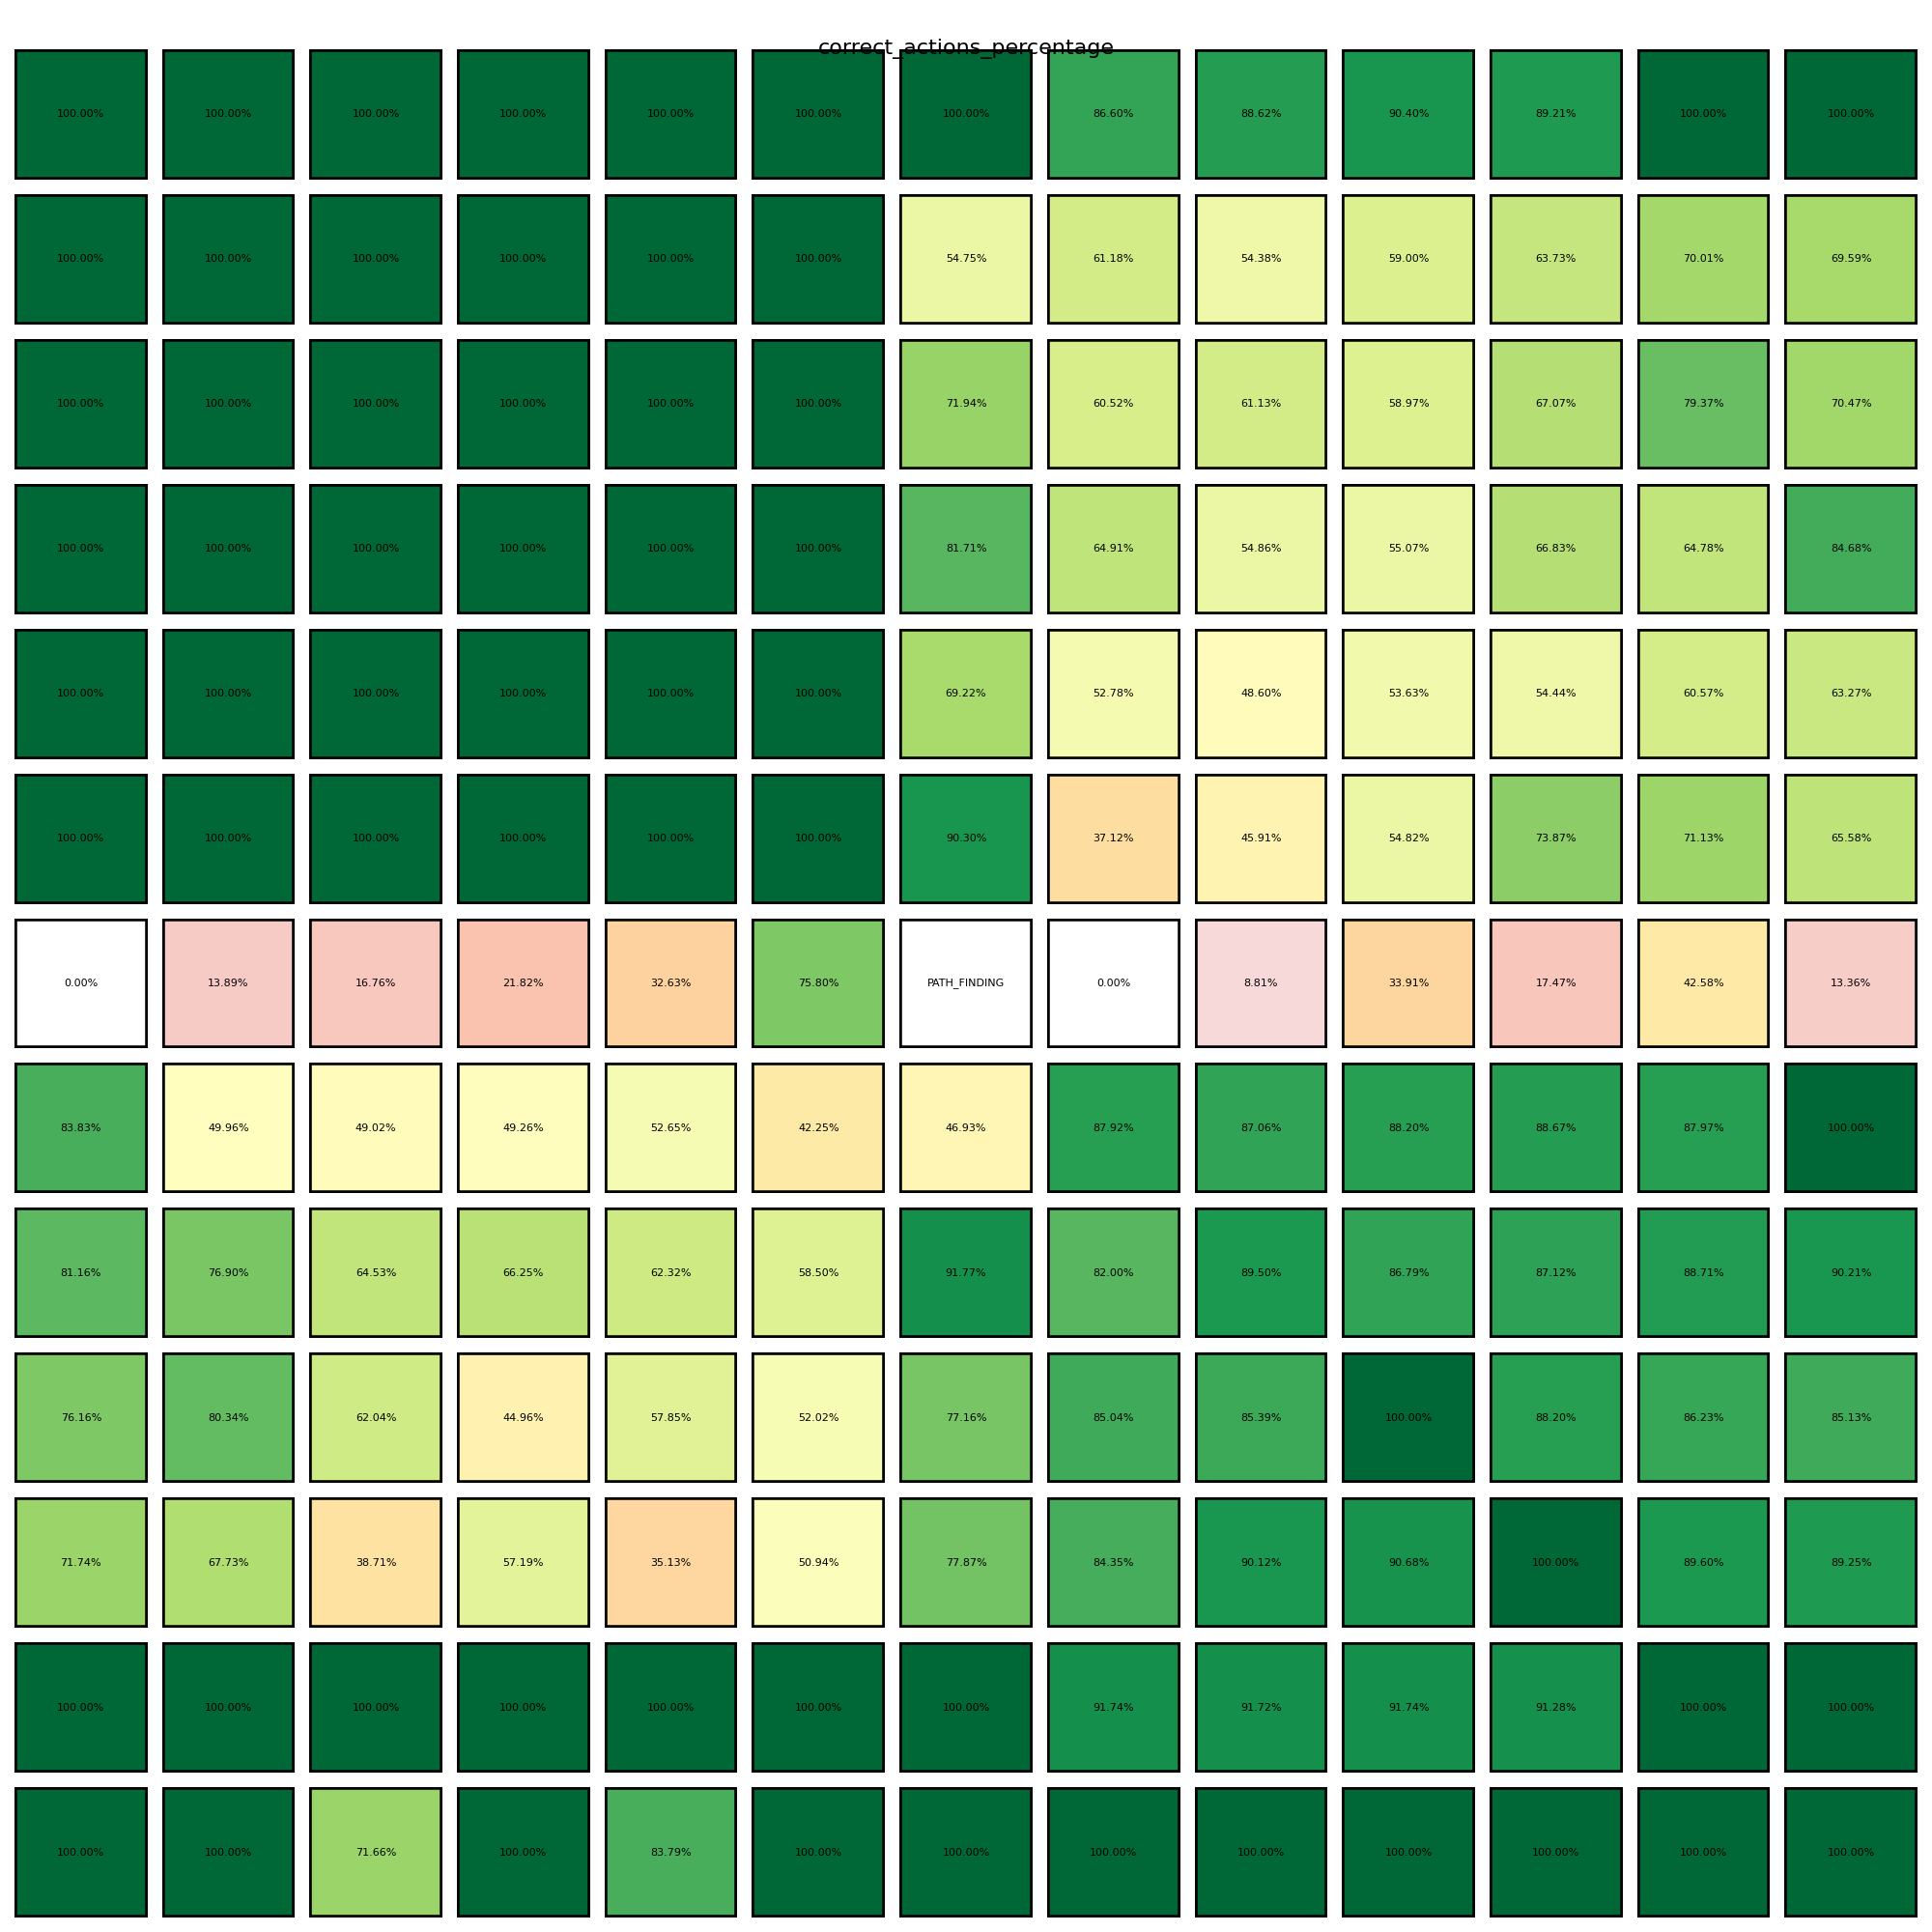
\includegraphics[width=\textwidth]{
      images/results_discussion/correctness_hm_TL.png
    }
    \caption{Top Left Origin Orientation}
    \label{fig:heatmapTL}
  \end{minipage}
  \caption{Correctness Heatmaps showing the percentage of correct actions in
  each cell}
  \label{fig:orientation_correctness}
\end{figure}
\vspace{5mm}

\subsection{Comparison of Orientations}

When comparing the two orientations, we found that in the top-left origin
version, 154 tiles had one of the correct actions as the most probable choice.
In contrast, in the bottom-left origin version, only 104 tiles had a correct
action as the highest-probability choice. The comparison between the two orientations
reveals a clear preference for the top-left origin. The model performed
significantly better when using this orientation, as shown by the following accuracy
metrics:
\begin{itemize}
  \item \textbf{Top-left origin}: 92\% of the tiles had the correct action as
    the most probable one;

  \item \textbf{Bottom-left origin}: 62\% of the tiles had the correct action as
    the most probable one;

  \item \textbf{Top 3 actions comparison}: 99\% vs. 93\% of the tiles contained
    the correct action within the top three choices.
\end{itemize}

These results strongly suggest that the model is inherently biased toward the top-left
origin orientation. This finding highlights the potential influence of data
structure representations on LLM-based decision-making and suggests that models
trained on structured data formats may develop spatial preferences that impact
their performance in spatial reasoning tasks.

\section{Stateless}
\label{sec:stateless}

As previously discussed in Section \ref{sec:stateful_and_stateless_agents_chapAD},
a stateless agent operates without any memory of past actions or previous states
of the environment. In this context, every decision is made independently, relying
solely on the information provided within a single prompt.

Technically, each call to the Large Language Model (LLM) contains only the
current state of the environment, without any reference to past states or prior actions.
For every decision, a new conversation instance is initiated, making the agent
unable to build an internal representation of the map or track past movements.

One of the major challenges faced by a stateless agent is the need to infer its
position and the map layout solely based on the current prompt. This limitation leads
to several difficulties, such as:
\begin{itemize}
  \item \textbf{Inability to Track Progress:} Since the agent does not retain
    memory, it cannot recognize previously visited locations, often resulting in
    repetitive movements or getting stuck in loops.

  \item \textbf{Increased Uncertainty:} The LLM must deduce the correct course
    of action based only on the available snapshot of the environment, leading to
    occasional misinterpretations.

  \item \textbf{Higher Error Rates:} Compared to a stateful approach, where an agent
    can accumulate knowledge over time, the stateless method is more prone to
    making incorrect decisions, especially in larger maps.
\end{itemize}

Despite these challenges, implementing a stateless agent serves as an important step
toward understanding the inherent uncertainty in LLM-based decision-making. The
results obtained from this approach provide a useful baseline for evaluating the
potential benefits of incorporating statefulness.

The stateless agent follows predefined prompt templates, as described in Sections
\ref{sub:pickup_prompt} and \ref{sub:deliver_prompt}. These prompts encapsulate
all the necessary information about the current state and available actions
within a single request.

To evaluate the performance of the stateless agent, we analyze heatmaps generated
from experiments on different map sizes. The following sections present the
results for various scenarios.

\subsection{Pickup Goal at the Center}
\label{sub:pickup_goal_at_the_center}

Figures \ref{fig:stateless_pickup_heatmaps} and \ref{fig:stateless_pickup_correctness}
illustrate the heatmaps for maps of sizes 5x5, 7x7, and 13x13, with the pickup
goal placed at the center.

\vspace{5mm}
\begin{figure}[h]
  \centering
  \begin{minipage}[b]{0.32\textwidth}
    \centering
    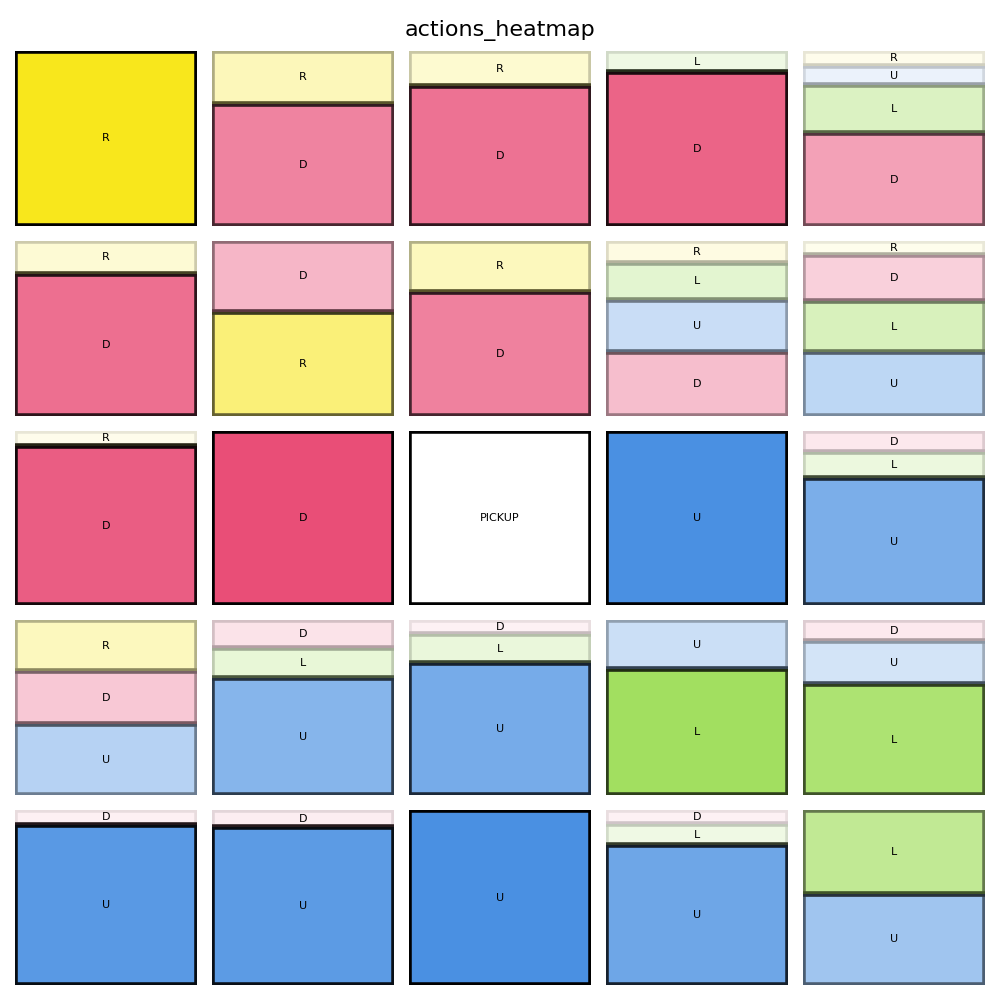
\includegraphics[width=\textwidth]{
      images/results_discussion/stateless/hm_5x5_pickup.png
    }
    \caption{5x5}
    \label{fig:hm_5x5_pickup}
  \end{minipage}
  \hfill
  \begin{minipage}[b]{0.32\textwidth}
    \centering
    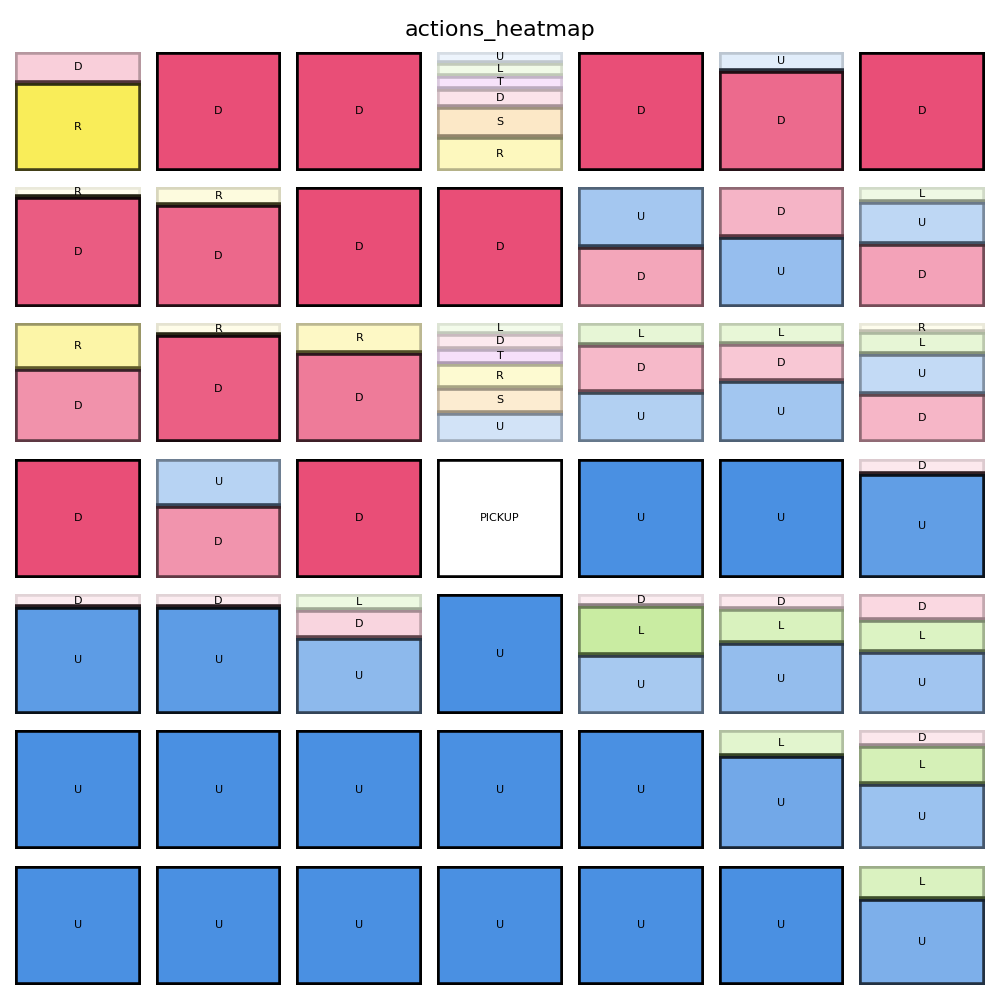
\includegraphics[width=\textwidth]{
      images/results_discussion/stateless/hm_7x7_pickup.png
    }
    \caption{7x7}
    \label{fig:hm_7x7_pickup}
  \end{minipage}
  \hfill
  \begin{minipage}[b]{0.32\textwidth}
    \centering
    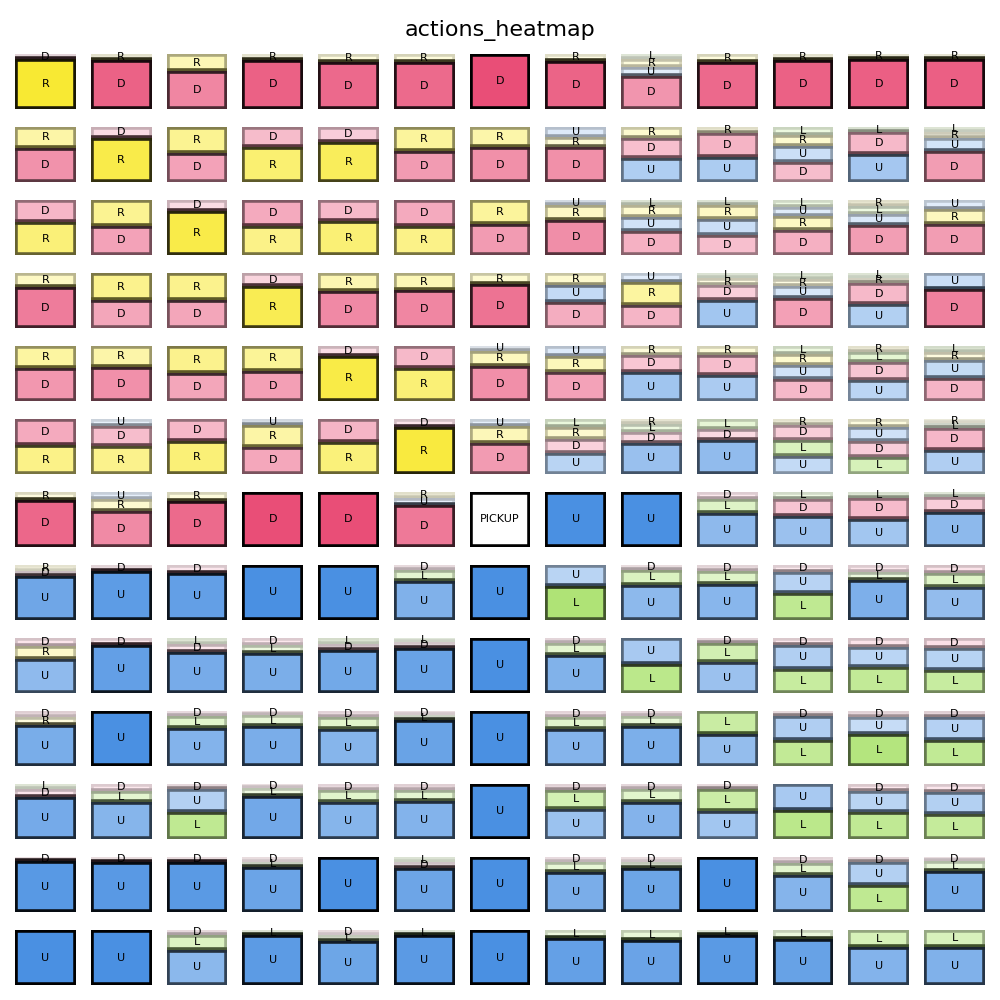
\includegraphics[width=\textwidth]{
      images/results_discussion/stateless/hm_13x13_pickup.png
    }
    \caption{13x13}
    \label{fig:hm_13x13_pickup}
  \end{minipage}
  \caption{Heatmaps for stateless agent with pickup goal in the center of
  different map sizes}
  \label{fig:stateless_pickup_heatmaps}
\end{figure}
\vspace{5mm}

From the heatmaps, we can observe a consistent pattern across different map
sizes. The top-left quadrant tends to show red and yellow as prominent colors and
the bottom-left quadrant is predominantly blue. The top-right quadrant exhibits
significant uncertainty with many actions in most of the cells, while the bottom-right
quadrant generally is green and blue (colors representing every actions, as explained
in Section \ref{sub:heatmaps}).

To further examine the correctness of the agent's decisions, we analyze the correctness
heatmaps shown in Figure \ref{fig:stateless_pickup_correctness}.

\vspace{5mm}
\begin{figure}[h]
  \centering
  \begin{minipage}[b]{0.32\textwidth}
    \centering
    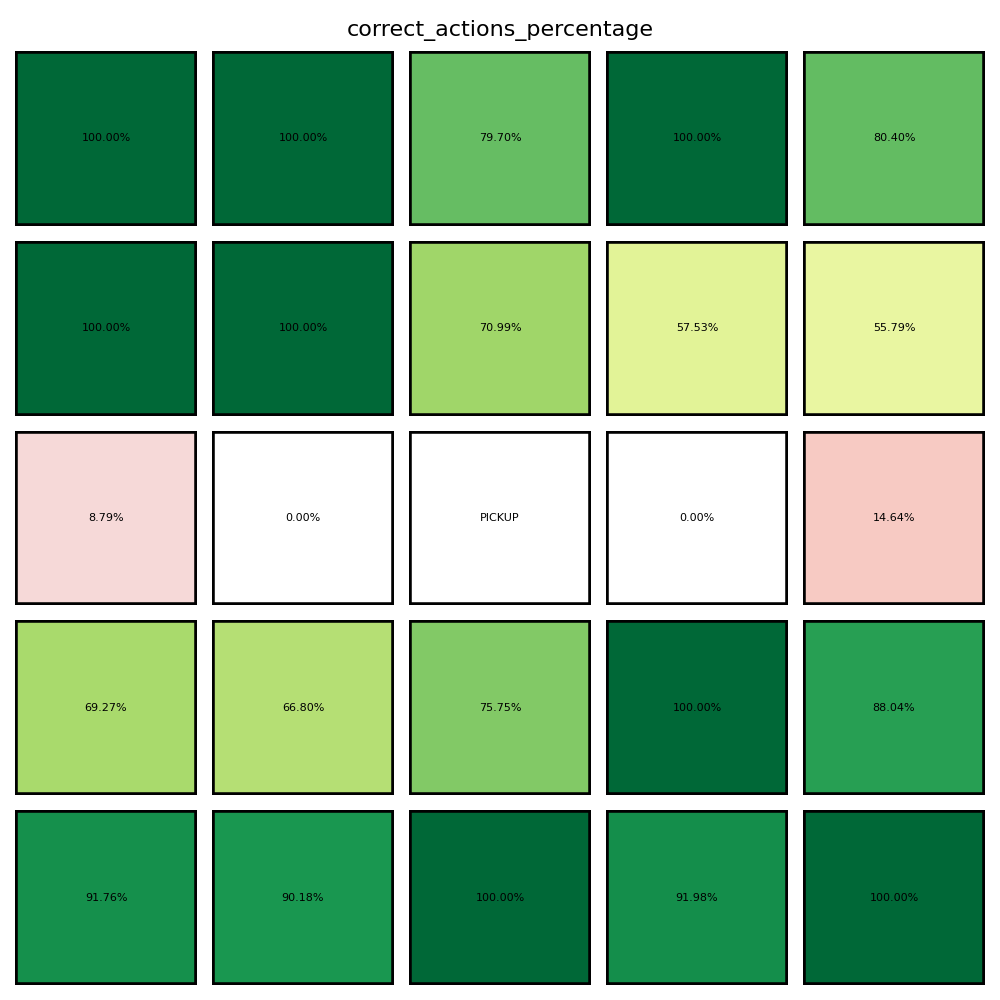
\includegraphics[width=\textwidth]{
      images/results_discussion/stateless/chm_5x5_pickup.png
    }
    \caption{5x5}
    \label{fig:chm_5x5_pickup}
  \end{minipage}
  \hfill
  \begin{minipage}[b]{0.32\textwidth}
    \centering
    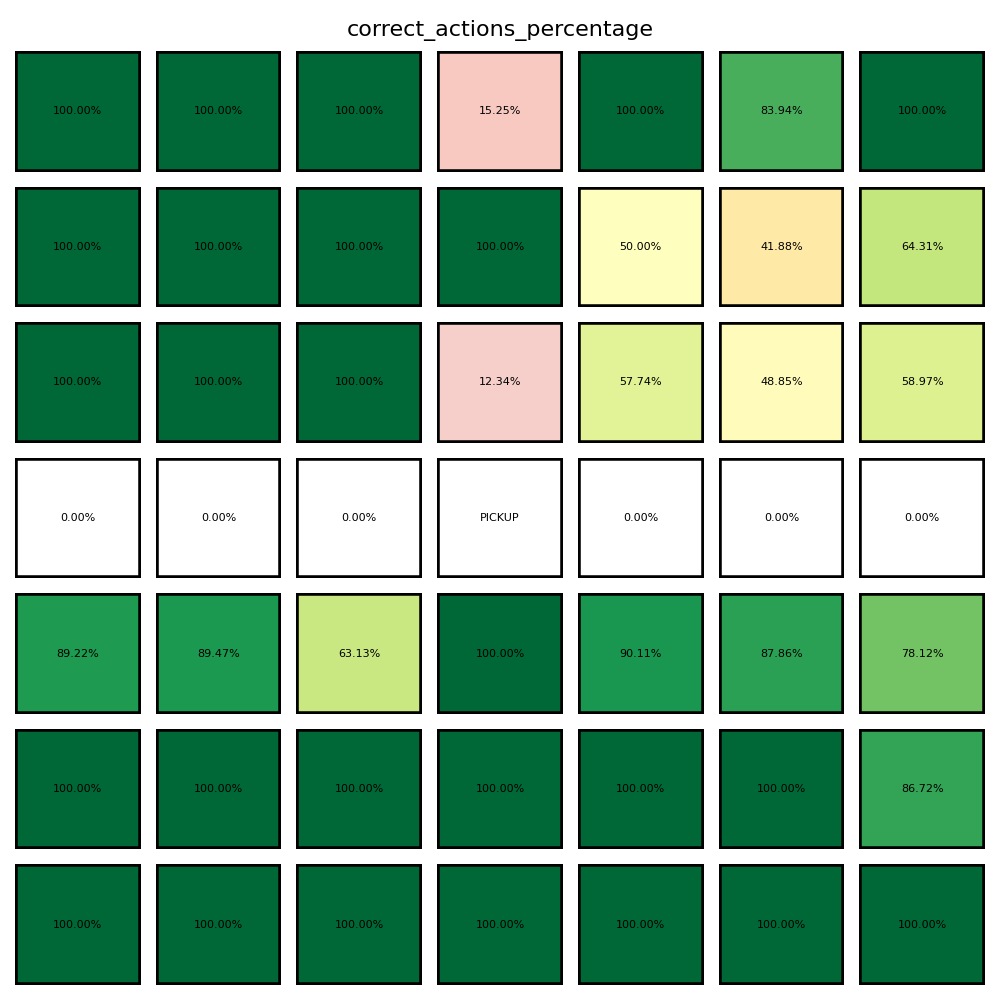
\includegraphics[width=\textwidth]{
      images/results_discussion/stateless/chm_7x7_pickup.png
    }
    \caption{7x7}
    \label{fig:chm_7x7_pickup}
  \end{minipage}
  \hfill
  \begin{minipage}[b]{0.32\textwidth}
    \centering
    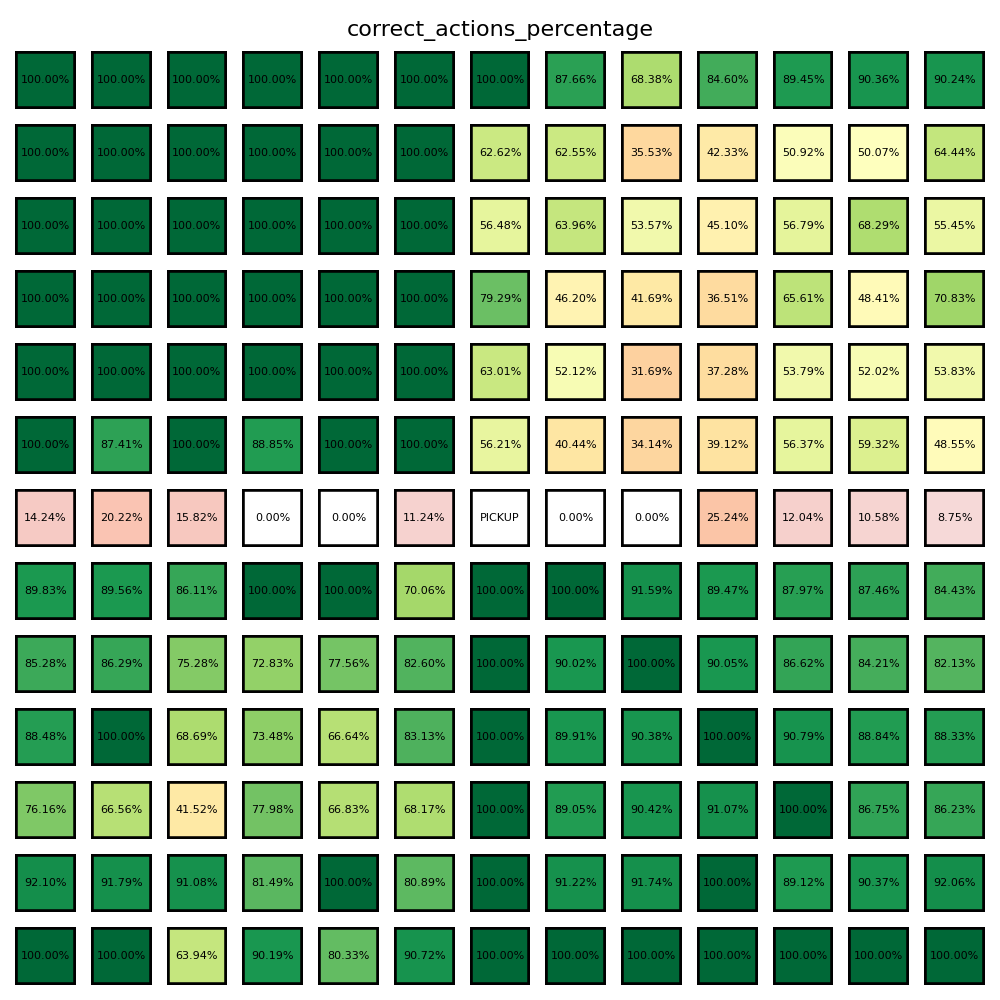
\includegraphics[width=\textwidth]{
      images/results_discussion/stateless/chm_13x13_pickup.png
    }
    \caption{13x13}
    \label{fig:chm_13x13_pickup}
  \end{minipage}
  \caption{Correctness heatmaps for stateless agent with pickup goal at the
  center of different map sizes.}
  \label{fig:stateless_pickup_correctness}
\end{figure}
\vspace{5mm}

The correctness analysis reveals the following trends:
\begin{itemize}
  \item The top-left and bottom-right quadrants exhibit the highest certainty,
    with the former being almost perfect in every cell;

  \item The top-right and bottom-left quadrants are more uncertain, with the top-right
    being the least reliable;

  \item Along the row and column containing the goal, the correctness tends to
    be lower, with several cells having 0\% correctness, meaning that the only correct
    action was discarded by KnowNo
\end{itemize}

Table \ref{tab:performance} presents numerical performance metrics across
different map sizes. The number of times the correct action is present in the $X$
actions with the highest probability is shown in the $topX$ columns, while their
percentage is in the $topX\%$ columns.

\vspace{5mm}
\begin{table}[h]
  \centering
  \begin{tabular}{c|ccc|ccc}
          & top1 & top2 & top3 & top1\% & top2\% & top3\% \\
    \hline
    5x5   & 19   & 22   & 22   & 0.792  & 0.917  & 0.917  \\
    7x7   & 37   & 40   & 41   & 0.771  & 0.833  & 0.854  \\
    13x13 & 125  & 161  & 162  & 0.744  & 0.958  & 0.964  \\
  \end{tabular}
  \caption{Performance metrics for different map sizes - pickup goal}
  \label{tab:performance}
\end{table}
\vspace{5mm}

The results indicate that:
\begin{itemize}
  \item Smaller maps tend to yield a higher probability of selecting the correct
    action as the top-ranked choice.

  \item While absolute correctness decreases with increasing map size, the
    relative performance remains fairly stable.
\end{itemize}

Even if not visible in the heatmaps, the goal tile almost always had the correct
action as the only one kept after KnowNo framework, and rarely it kept other actions
but the correct one had a better probability by far. Only in one case, the ``goal
action" was the most probable also in the left cell wrt the goal.

\subsection{Deliver Goal at the Center}

A similar analysis can be conducted for the case where the delivery goal is placed
at the center of the map. Figures \ref{fig:stateless_deliver_heatmaps} and
\ref{fig:stateless_deliver_correctness} show the heatmaps for different map
sizes in this configuration.

Compared to the pickup task, the delivery task introduces slightly more uncertainty.
This uncertainty arises because, in our setup, the goal tile is not explicitly
marked as a destination in the prompt but must instead be inferred from the map
description. Again, the LLM needs to recognize that it has arrived at the
correct location based solely on relative positioning within the map, without any
persistent memory of past decisions.

From the heatmaps, we observe similar trends as seen in the pickup case:
\begin{itemize}
  \item The top-left and bottom-right quadrants show a higher concentration of correct
    probability;

  \item The top-right quadrant, similar to the pickup scenario, exhibits more variability
    and uncertainty;

  \item The row and column containing the goal continue to demonstrate reduced correctness.
\end{itemize}

\vspace{5mm}
\begin{figure}[h!]
  \centering
  \begin{minipage}[b]{0.32\textwidth}
    \centering
    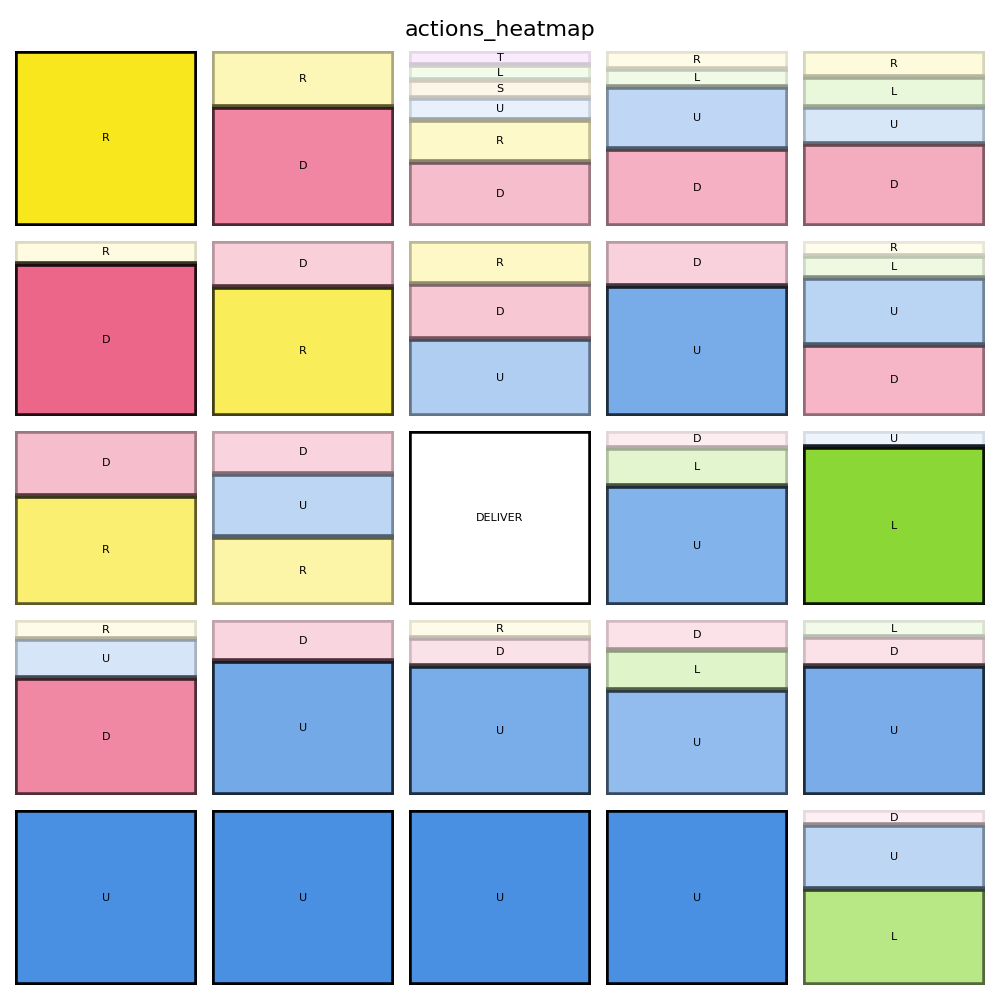
\includegraphics[width=\textwidth]{
      images/results_discussion/stateless/hm_5x5_deliver.png
    }
    \caption{5x5}
    \label{fig:hm_5x5_deliver}
  \end{minipage}
  \hfill
  \begin{minipage}[b]{0.32\textwidth}
    \centering
    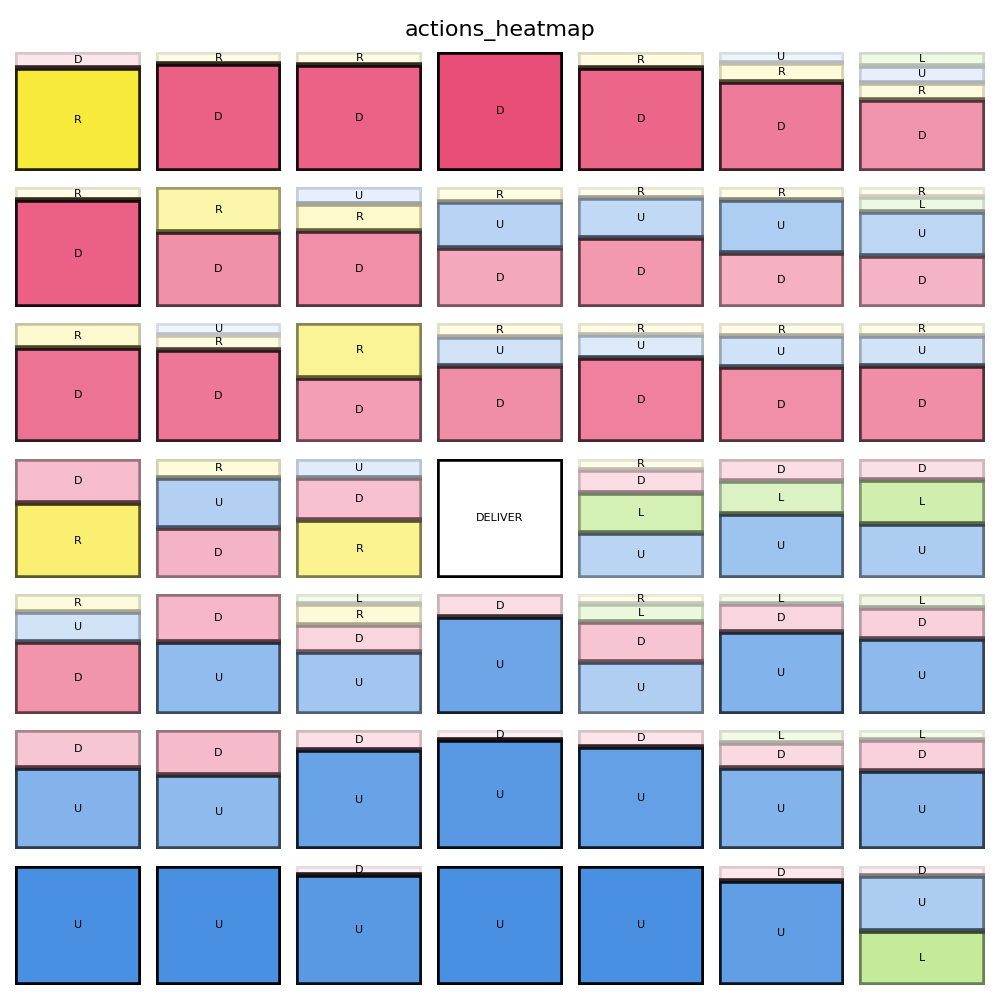
\includegraphics[width=\textwidth]{
      images/results_discussion/stateless/hm_7x7_deliver.png
    }
    \caption{7x7}
    \label{fig:hm_7x7_deliver}
  \end{minipage}
  \hfill
  \begin{minipage}[b]{0.32\textwidth}
    \centering
    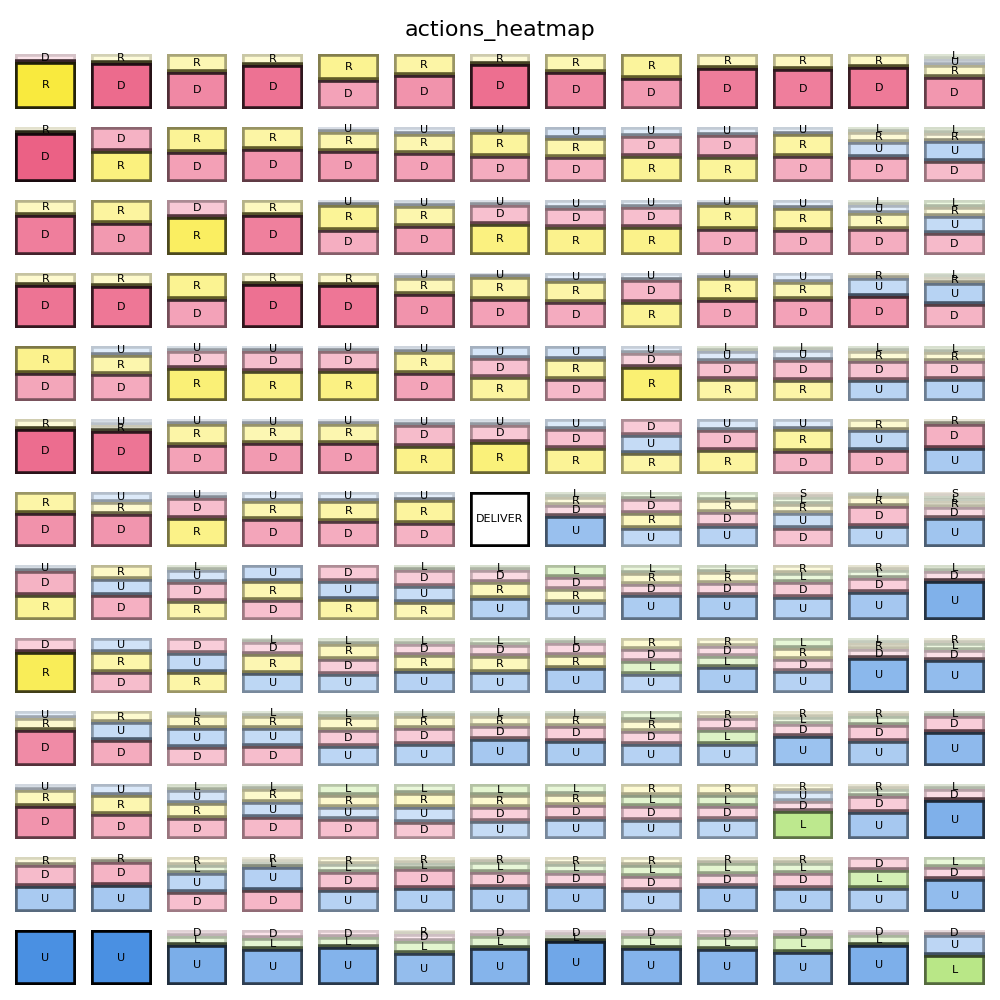
\includegraphics[width=\textwidth]{
      images/results_discussion/stateless/hm_13x13_deliver.png
    }
    \caption{13x13}
    \label{fig:hm_13x13_deliver}
  \end{minipage}
  \caption{Heatmaps for stateless agent with deliver goal in the center of
  different map sizes}
  \label{fig:stateless_deliver_heatmaps}
\end{figure}
\vspace{5mm}

\vspace{5mm}
\begin{figure}[h!]
  \centering
  \begin{minipage}[b]{0.32\textwidth}
    \centering
    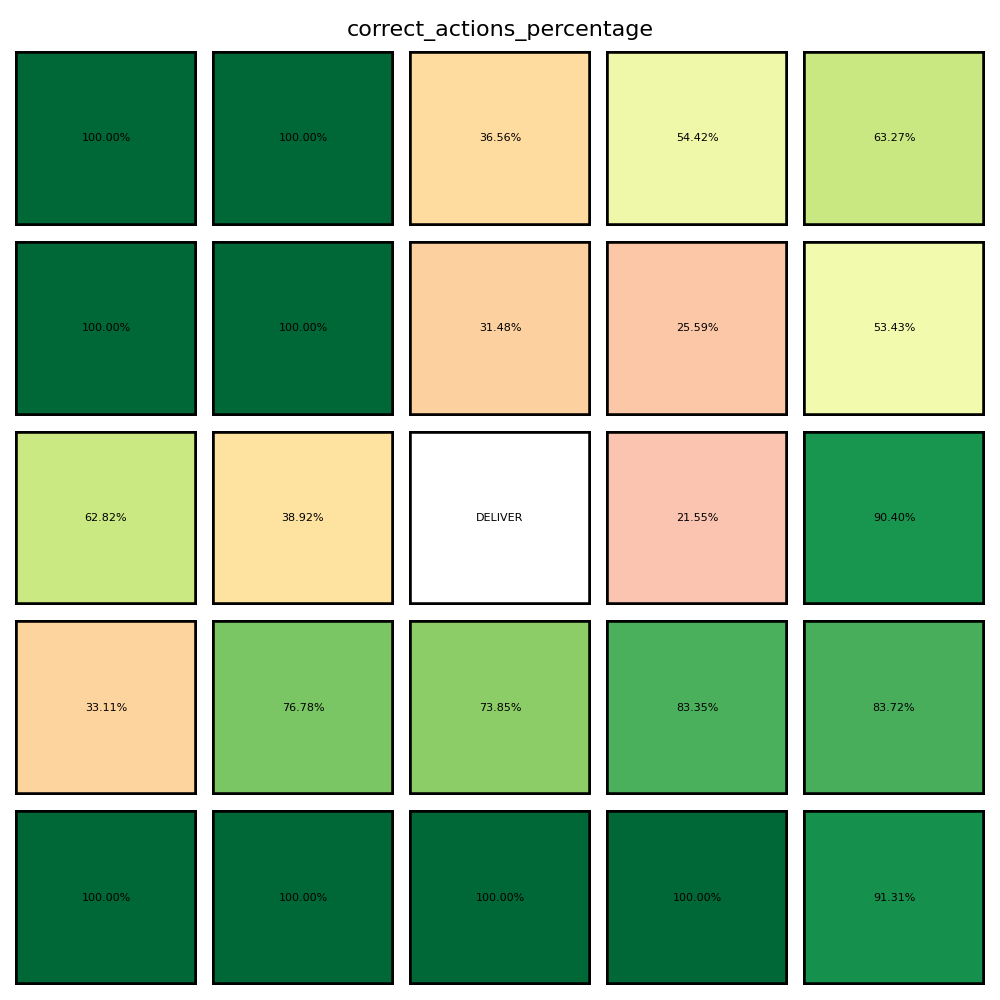
\includegraphics[width=\textwidth]{
      images/results_discussion/stateless/chm_5x5_deliver.png
    }
    \caption{5x5}
    \label{fig:chm_5x5_deliver}
  \end{minipage}
  \hfill
  \begin{minipage}[b]{0.32\textwidth}
    \centering
    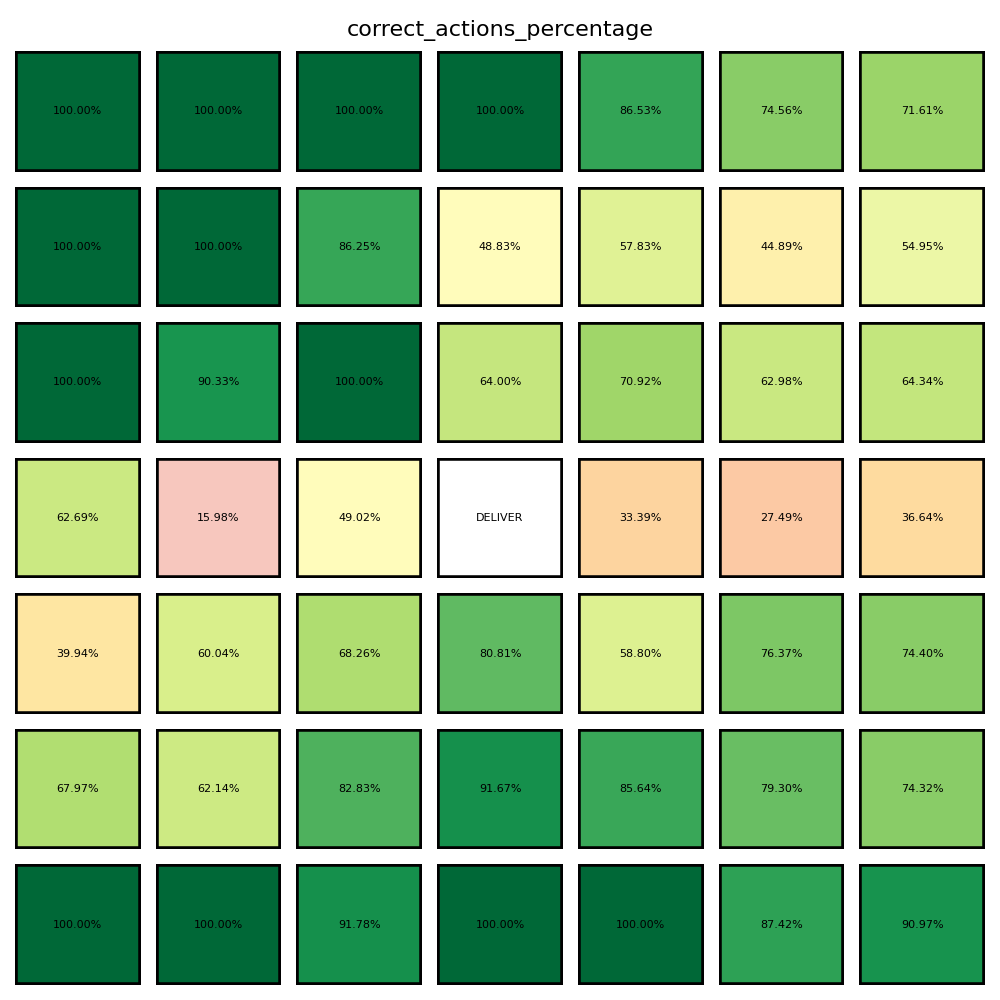
\includegraphics[width=\textwidth]{
      images/results_discussion/stateless/chm_7x7_deliver.png
    }
    \caption{7x7}
    \label{fig:chm_7x7_deliver}
  \end{minipage}
  \hfill
  \begin{minipage}[b]{0.32\textwidth}
    \centering
    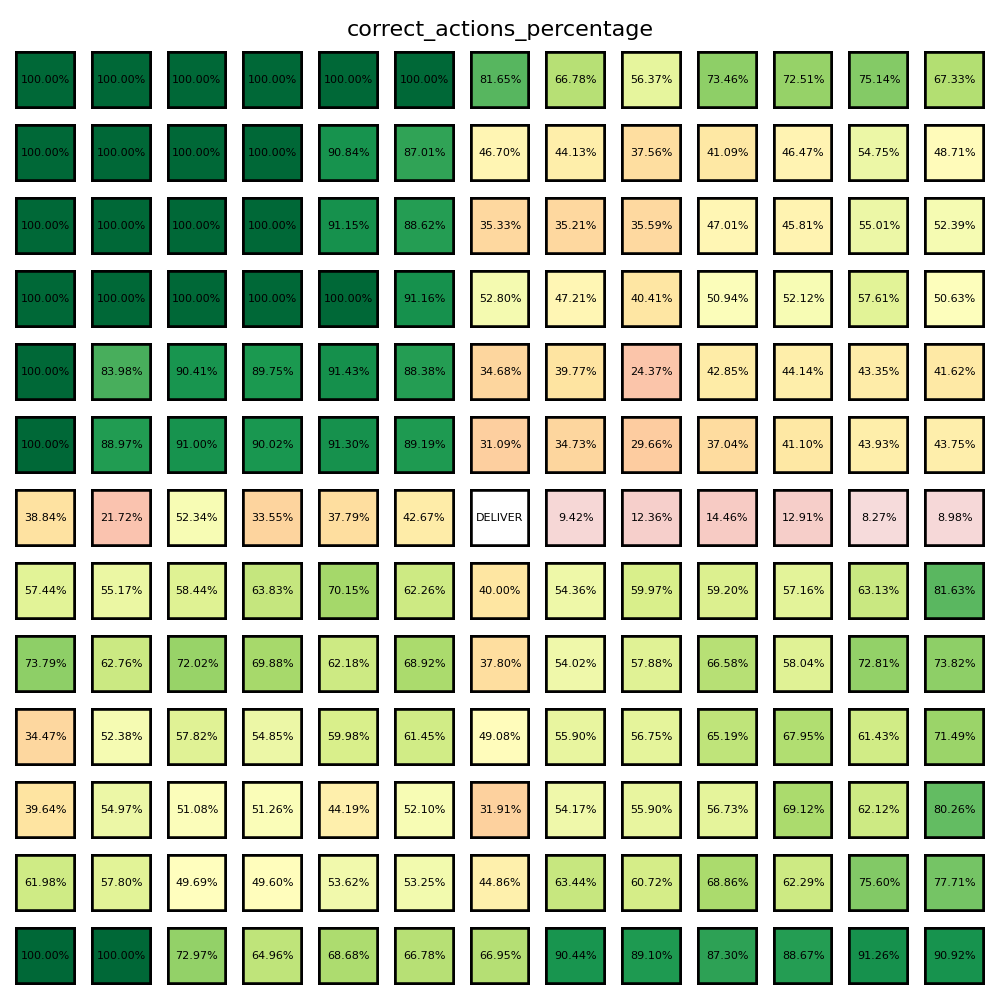
\includegraphics[width=\textwidth]{
      images/results_discussion/stateless/chm_13x13_deliver.png
    }
    \caption{13x13}
    \label{fig:chm_13x13_deliver}
  \end{minipage}
  \caption{Heatmaps for stateless agent with deliver goal in the center of
  different map sizes}
  \label{fig:stateless_deliver_correctness}
\end{figure}
\vspace{5mm}

Moreover, the values in Table \ref{tab:performance} reveals that as the map size
increases, the probability of selecting the correct action as the top-ranked
choice decreases. However, the overall trend remains consistent, suggesting that
while uncertainty increases with map size, the general patterns of decision-making
remain largely stable across different scales.

\vspace{5mm}
\begin{table}[h!]
  \centering
  \begin{tabular}{c|ccc|ccc}
          & top1 & top2 & top3 & top1\% & top2\% & top3\% \\
    \hline
    5x5   & 20   & 24   & 24   & 0.833  & 1.000  & 1.000  \\
    7x7   & 43   & 47   & 48   & 0.896  & 0.979  & 1.000  \\
    13x13 & 125  & 161  & 162  & 0.744  & 0.958  & 0.964  \\
  \end{tabular}
  \caption{Performance metrics for different map sizes - deliver goal}
  \label{tab:performance}
\end{table}
\vspace{5mm}

\subsection{Pickup and Deliver Goals in Different Map Sections}

Beyond testing the performance of the stateless agent scenarios with the goal at
the center, we also examined its ability to handle pickup and delivery goals positioned
in different sections of the map. Figures \ref{fig:stateless_top_right} and
\ref{fig:stateless_bottom_right} illustrate the heatmaps for cases where the
pickup and delivery locations are in the top-right and bottom-right corners, respectively.

By analyzing the performance in these different regions, we aim to understand
whether the placement of the goal influences the decision-making accuracy of the
LLM. Since the map is embedded within a structured text prompt, the location of
the goal may impact how the LLM processes the spatial relationships between
different tiles as explained in Section \ref{sub:goal_positioning}.

\vspace{5mm}
\begin{figure}[h!]
  \centering
  \begin{minipage}[b]{0.45\textwidth}
    \centering
    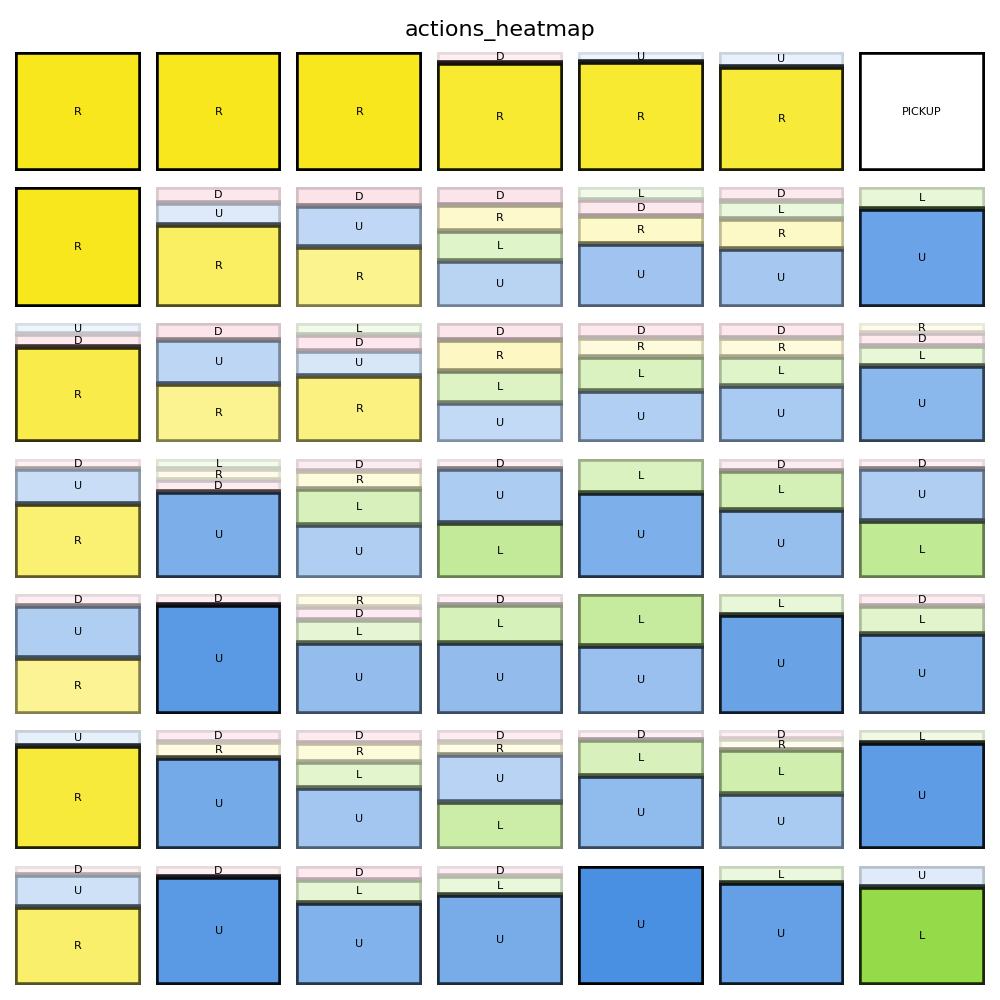
\includegraphics[width=\textwidth]{
      images/results_discussion/stateless/not_central/stateless_pickup_top_right.png
    }
    \caption{Pickup Top Right}
    \label{fig:stateless_pickup_top_right}
  \end{minipage}
  \hfill
  \begin{minipage}[b]{0.45\textwidth}
    \centering
    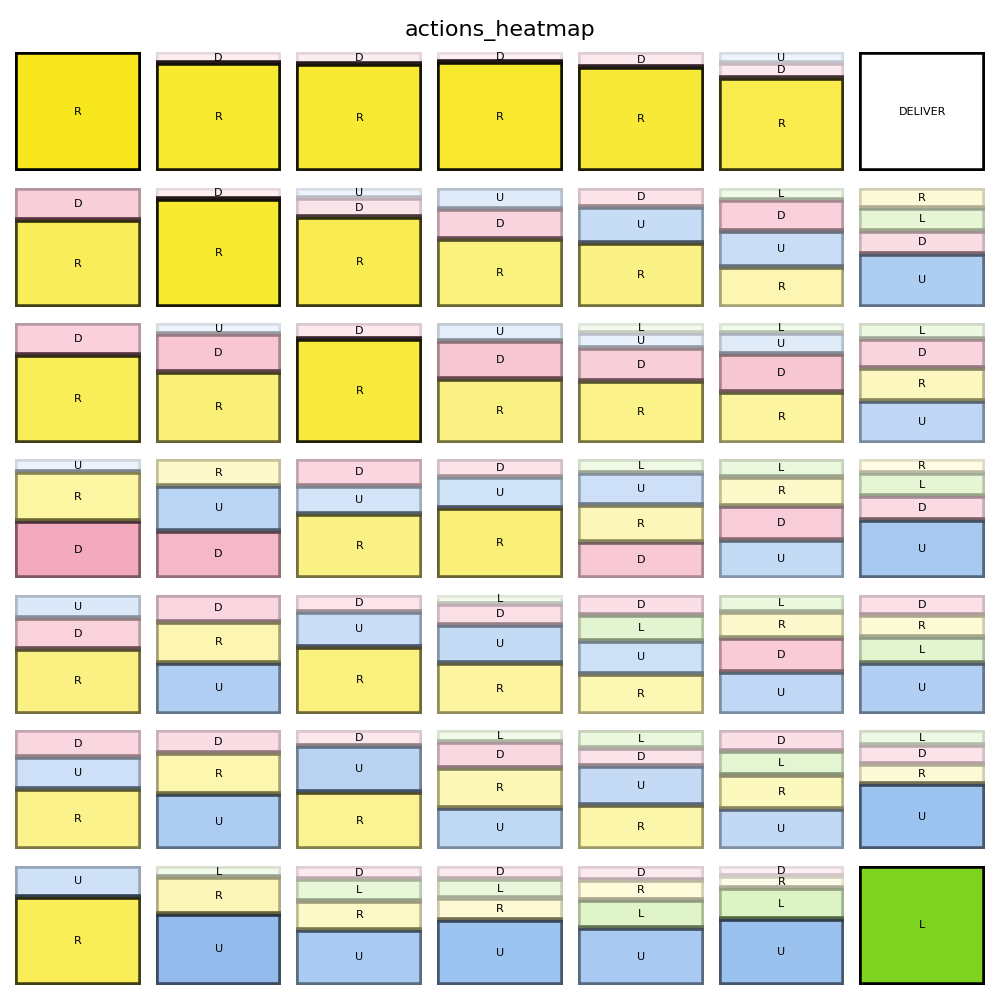
\includegraphics[width=\textwidth]{
      images/results_discussion/stateless/not_central/stateless_deliver_top_right.png
    }
    \caption{Deliver Top Right}
    \label{fig:stateless_deliver_top_right}
  \end{minipage}
  \caption{Heatmaps for stateless agent with pickup and deliver goals in the top
  right corner of the map}
  \label{fig:stateless_top_right}
\end{figure}
\vspace{5mm}

\begin{figure}[h!]
  \centering
  \begin{minipage}[b]{0.45\textwidth}
    \centering
    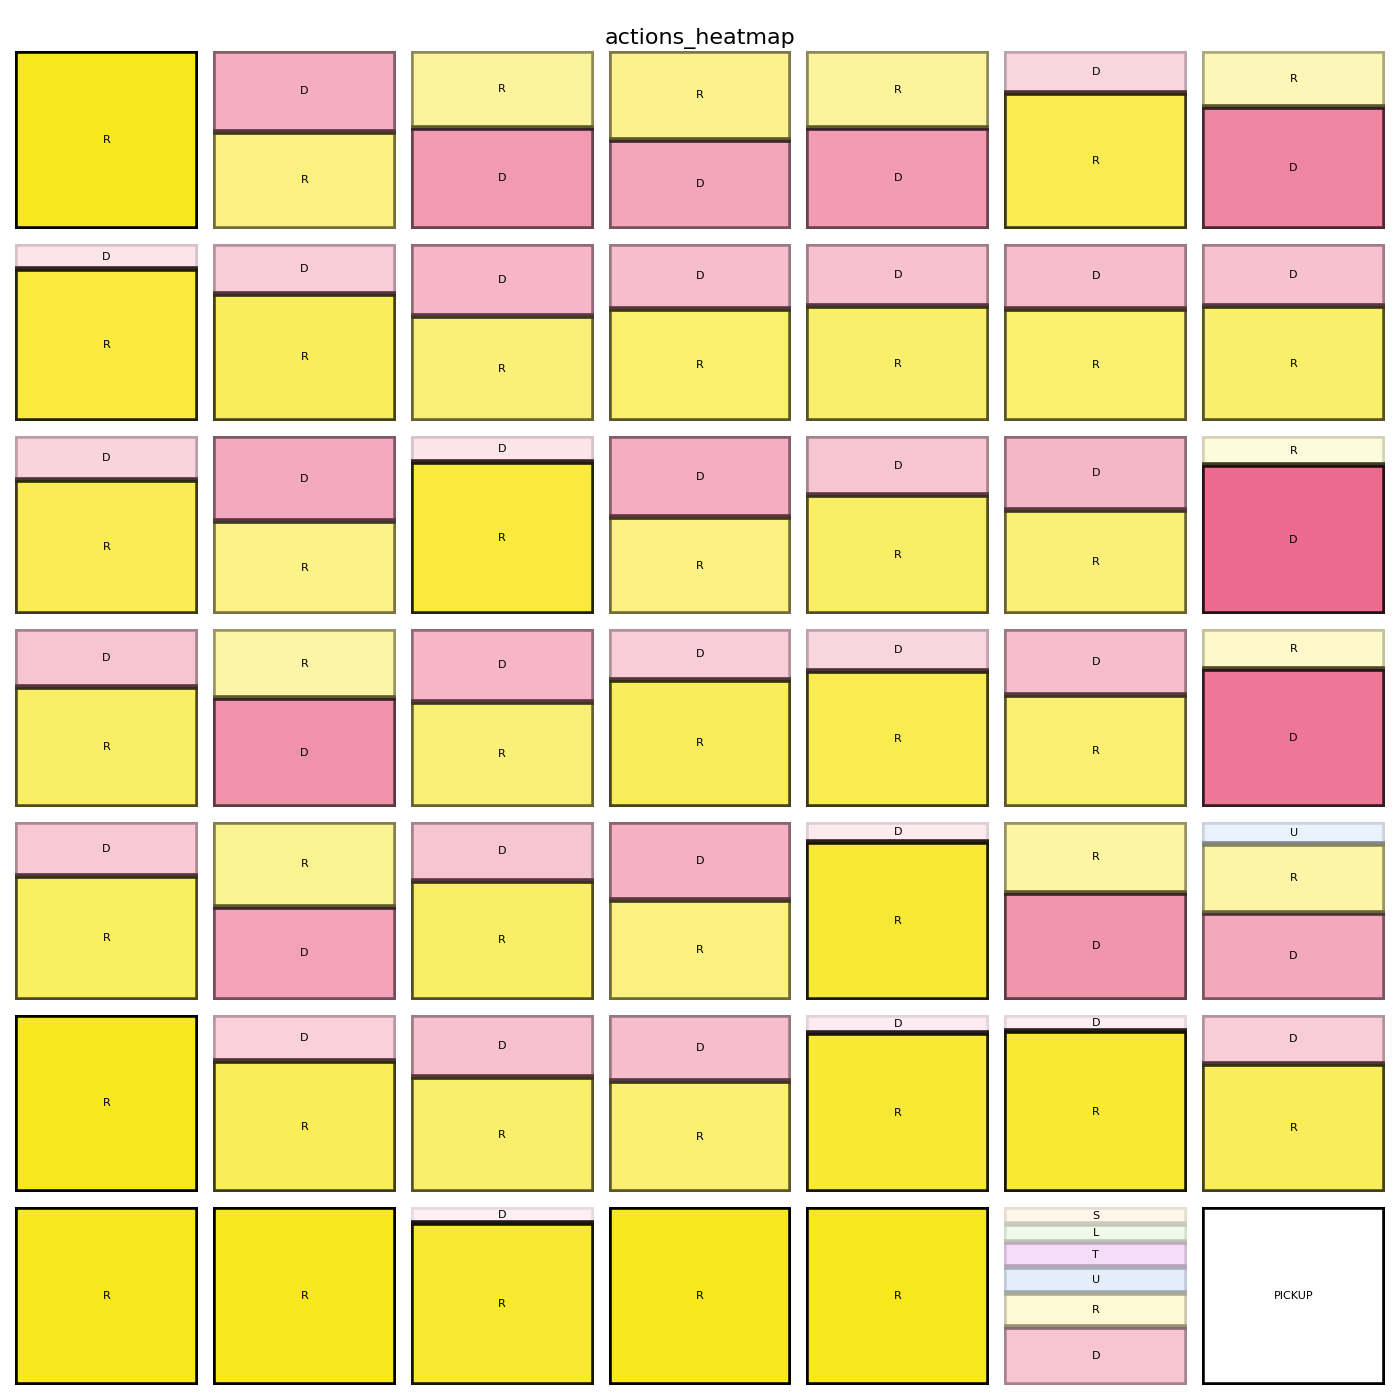
\includegraphics[width=\textwidth]{
      images/results_discussion/stateless/not_central/stateless_pickup_bottom_right.png
    }
    \caption{Pickup Bottom Right}
    \label{fig:stateless_pickup_bottom_right}
  \end{minipage}
  \hfill
  \begin{minipage}[b]{0.45\textwidth}
    \centering
    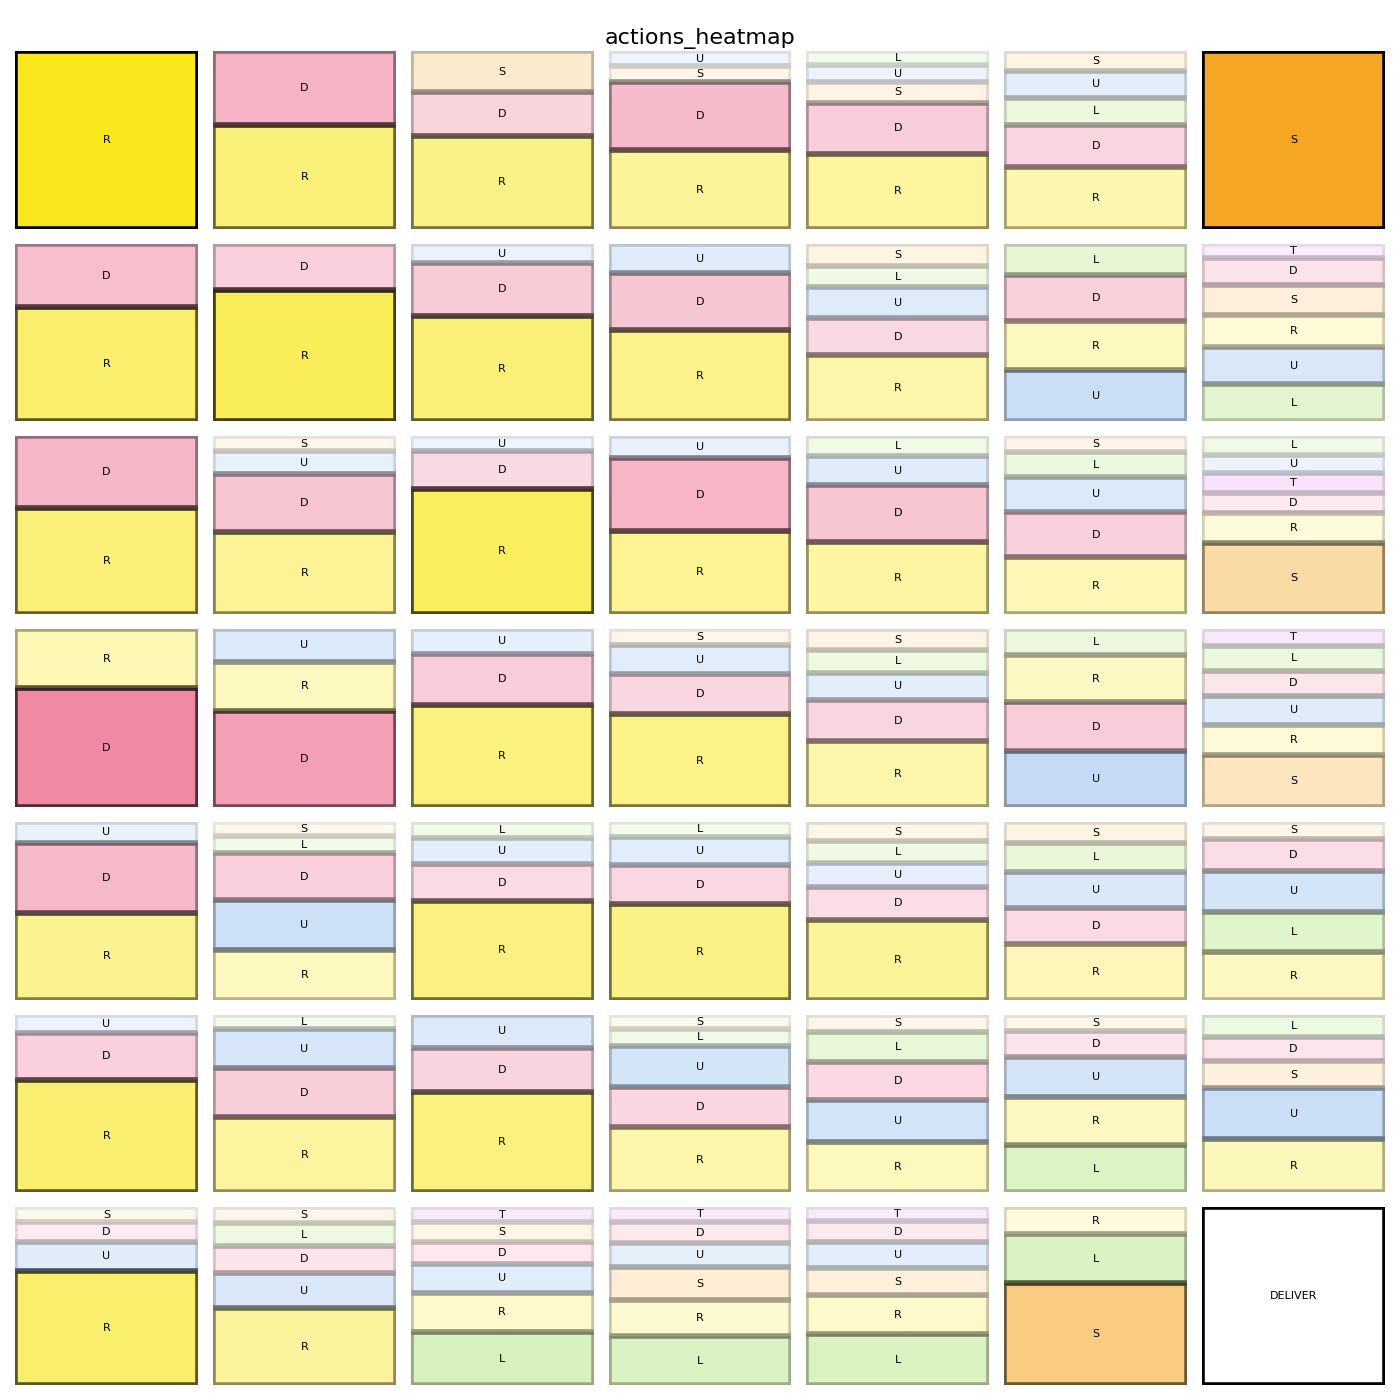
\includegraphics[width=\textwidth]{
      images/results_discussion/stateless/not_central/stateless_deliver_bottom_right.png
    }
    \caption{Deliver Bottom Right}
    \label{fig:stateless_deliver_bottom_right}
  \end{minipage}
  \caption{Heatmaps for stateless agent with pickup and deliver goals in the
  bottom right corner of the map}
  \label{fig:stateless_bottom_right}
\end{figure}
\vspace{5mm}

Looking at the correctness heatmaps in Figures
\ref{fig:stateless_top_right_correctness} and
\ref{fig:stateless_bottom_right_correctness}, we observe similar patterns, where
the characteristic drop in correctness along the goal row and column persists.

\vspace{5mm}
\begin{figure}[h]
  \centering
  \begin{minipage}[b]{0.45\textwidth}
    \centering
    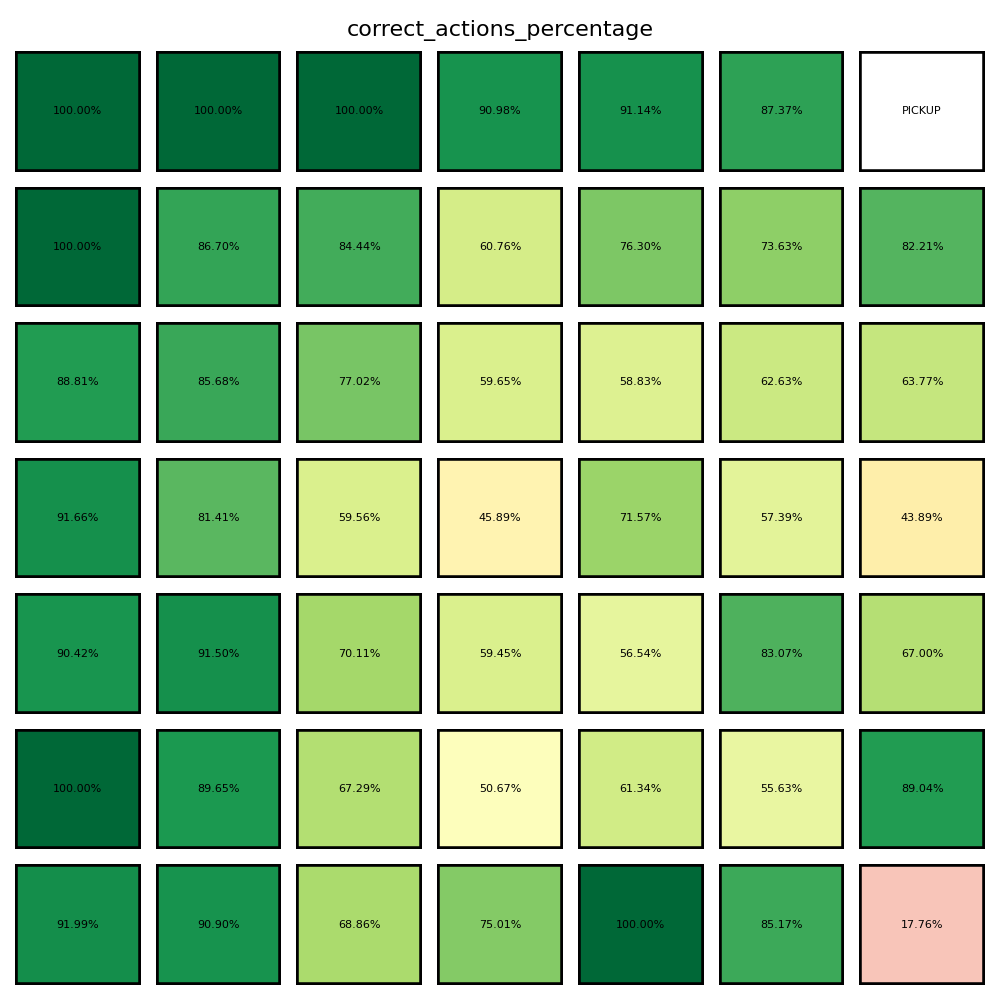
\includegraphics[width=\textwidth]{
      images/results_discussion/stateless/not_central/chm_pickup_top_right.png
    }
    \caption{Correctness Pickup Top Right}
    \label{fig:chm_pickup_top_right}
  \end{minipage}
  \hfill
  \begin{minipage}[b]{0.45\textwidth}
    \centering
    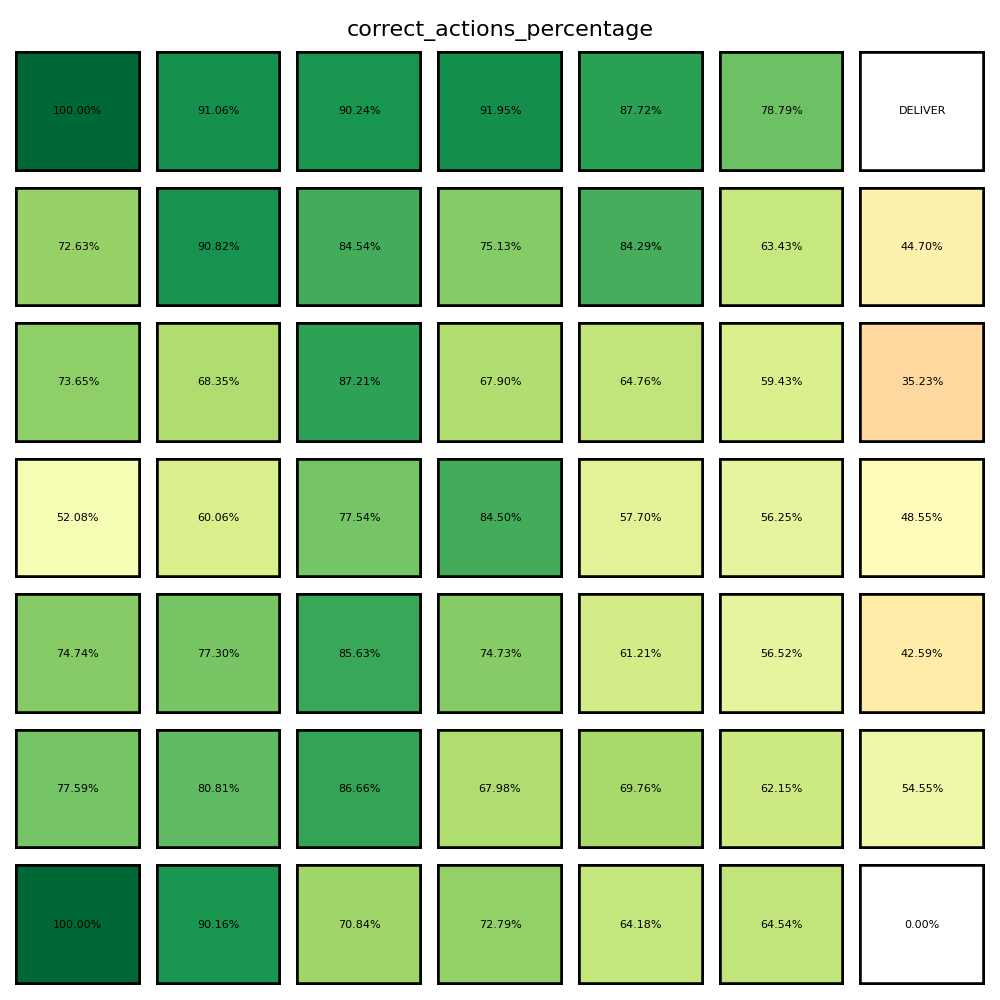
\includegraphics[width=\textwidth]{
      images/results_discussion/stateless/not_central/chm_deliver_top_right.png
    }
    \caption{Correctness Deliver Top Right}
    \label{fig:chm_deliver_top_right}
  \end{minipage}
  \caption{Correctness heatmaps for stateless agent with pickup and deliver
  goals in the top right corner of the map}
  \label{fig:stateless_top_right_correctness}
\end{figure}
\vspace{5mm}

\vspace{5mm}
\begin{figure}[h]
  \centering
  \begin{minipage}[b]{0.45\textwidth}
    \centering
    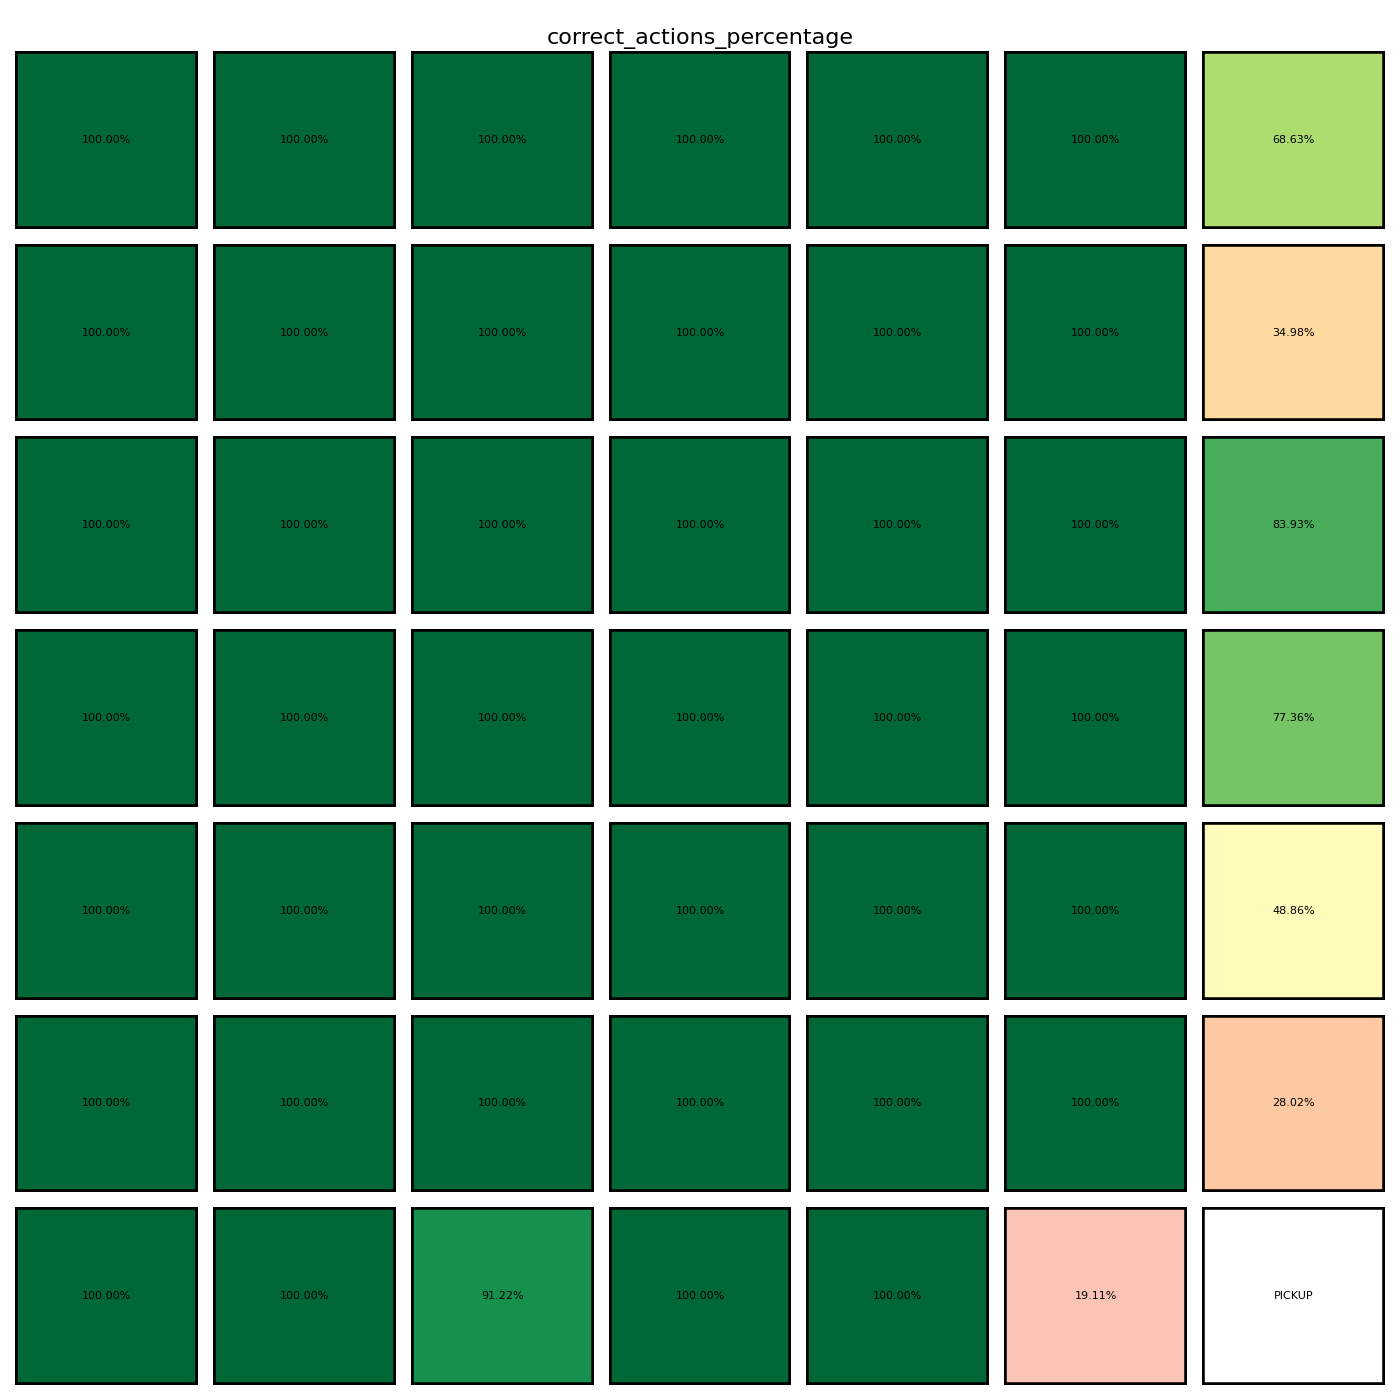
\includegraphics[width=\textwidth]{
      images/results_discussion/stateless/not_central/chm_pickup_bottom_right.png
    }
    \caption{Correctness Pickup Bottom Right}
    \label{fig:chm_pickup_bottom_right}
  \end{minipage}
  \hfill
  \begin{minipage}[b]{0.45\textwidth}
    \centering
    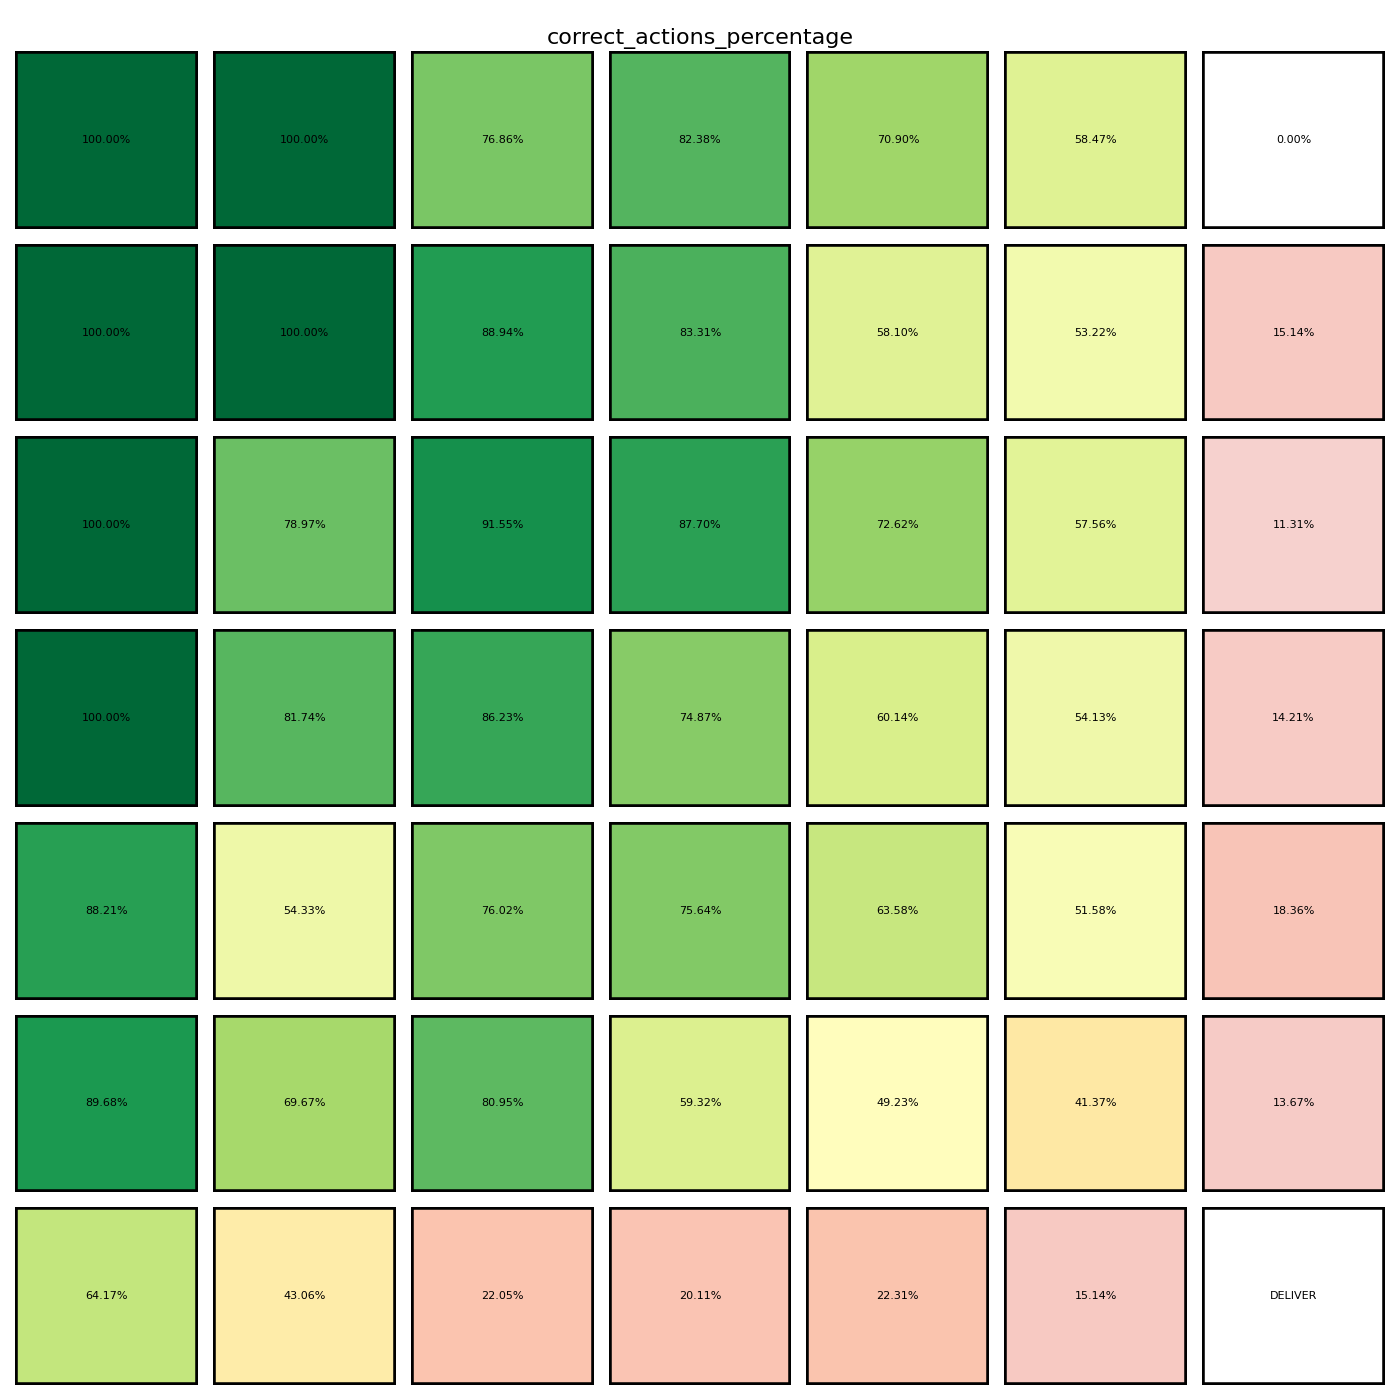
\includegraphics[width=\textwidth]{
      images/results_discussion/stateless/not_central/chm_deliver_bottom_right.png
    }
    \caption{Correctness Deliver Bottom Right}
    \label{fig:chm_deliver_bottom_right}
  \end{minipage}
  \caption{Correctness heatmaps for stateless agent with pickup and deliver
  goals in the bottom right corner of the map}
  \label{fig:stateless_bottom_right_correctness}
\end{figure}
\vspace{5mm}

These alternative goal placements provide valuable insights into the agent's
decision-making and can be seen as subsets of the larger map. For example, the
top-left portion of a 13x13 map with the goal in the center can be viewed as a
7x7 map with the goal in the bottom-right cell. At the same time, the bottom-left
portion of the 13x13 map with the center goal corresponds to a 7x7 map with the
top-right goal. This perspective brings us to the following topic, where a slice
with the same size from different maps is compared.

\vspace{5mm}
\begin{figure}[h]
  \centering
  \begin{minipage}[b]{0.19\textwidth}
    \centering
    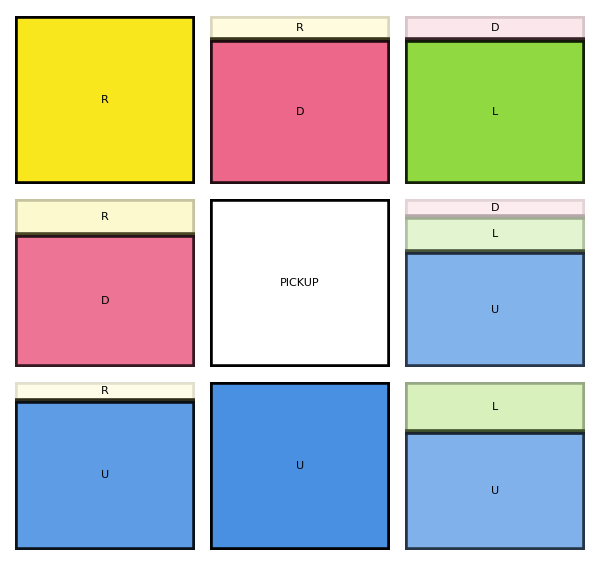
\includegraphics[width=\textwidth]{
      images/results_discussion/comparison/hm_3x3.png
    }
    \caption{3x3}
    \label{fig:hm_3x3}
  \end{minipage}
  \hfill
  \begin{minipage}[b]{0.19\textwidth}
    \centering
    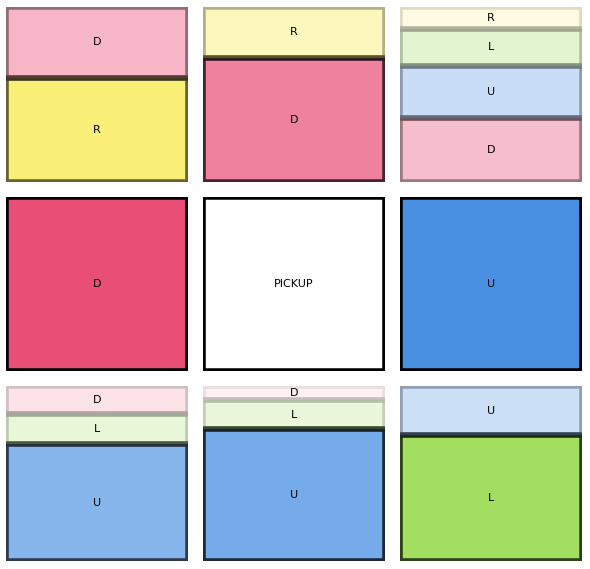
\includegraphics[width=\textwidth]{
      images/results_discussion/comparison/hm_5x5.png
    }
    \caption{5x5}
    \label{fig:hm_5x5}
  \end{minipage}
  \hfill
  \begin{minipage}[b]{0.19\textwidth}
    \centering
    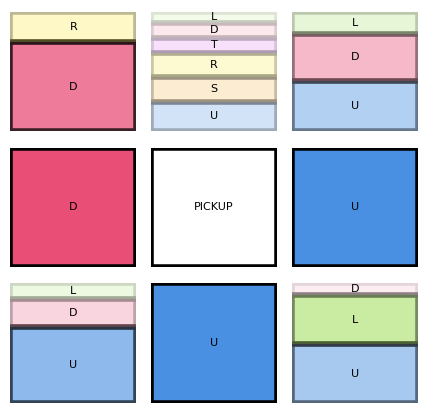
\includegraphics[width=\textwidth]{
      images/results_discussion/comparison/hm_7x7.png
    }
    \caption{7x7}
    \label{fig:hm_7x7}
  \end{minipage}
  \hfill
  \begin{minipage}[b]{0.19\textwidth}
    \centering
    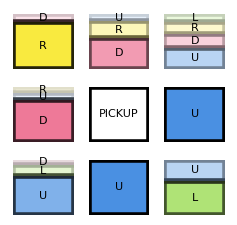
\includegraphics[width=\textwidth]{
      images/results_discussion/comparison/hm_13x13.png
    }
    \caption{13x13}
    \label{fig:hm_13x13}
  \end{minipage}
  \hfill
  \begin{minipage}[b]{0.19\textwidth}
    \centering
    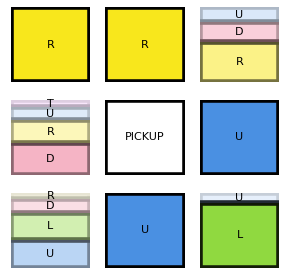
\includegraphics[width=\textwidth]{
      images/results_discussion/comparison/hm_21x21.png
    }
    \caption{21x21}
    \label{fig:hm_21x21}
  \end{minipage}
  \caption{Heatmaps of the 8 tiles around the goal for different map sizes}
  \label{fig:around_comparison}
\end{figure}
\vspace{5mm}

It is already visible in figure \ref{fig:stateless_deliver_heatmaps} but can be seen
better in figure \ref{fig:around_comparison}. Even if the values in the cells
around the goal are very similar, they are not the same. This may be due to the
fact that the LLM spreads the attention across all the prompt, and with a smaller
map, the map occupies less space in it.

\subsection{Goal position comparison}

A final analysis was conducted to determine whether the placement of the delivery
goal in different sections of the map affects the overall accuracy of the stateless
agent. Table \ref{tab:performance_21x21} presents performance metrics for the
21x21 grid in three configurations:
\begin{itemize}
  \item \textbf{Top Right (TR):} The delivery goal is positioned in the top-right
    corner;

  \item \textbf{Center (CN):} The delivery goal is placed in the center of the
    map;

  \item \textbf{Bottom Right (BR):} The delivery goal is located in the bottom-right
    corner.
\end{itemize}

\begin{table}[h]
  \centering
  \begin{tabular}{c|ccc|ccc}
              & top1 & top2 & top3 & top1\% & top2\% & top3\% \\
    \hline
    21x21\_TR & 378  & 429  & 433  & 0.859  & 0.975  & 0.984  \\
    21x21\_CN & 294  & 394  & 428  & 0.668  & 0.895  & 0.973  \\
    21x21\_BR & 371  & 416  & 417  & 0.843  & 0.945  & 0.948  \\
  \end{tabular}
  \caption{Performance metrics for different 21x21 configurations}
  \label{tab:performance_21x21}
\end{table}

From the data, we can draw several conclusions:
\begin{itemize}
  \item The top-right and bottom-right configurations exhibit similar performance,
    with top1 accuracy at 85.9\% and 84.3\%, respectively, as stated in Section
    \ref{sub:goal_positioning};

  \item The center goal configuration shows a notable drop in top1 accuracy to 66.8\%,
    confirming our earlier observation that finding a specific information hidden
    in the middle of a long text is more challenging;

  \item The difference between the top2 and top3 accuracy rates across the three
    configurations indicates that, even when the correct action is not the most
    probable choice, it is still frequently within the top-ranked options,
    meaning the model maintains a reasonable degree of decision-making
    reliability.
\end{itemize}

These results reinforce the hypothesis that stateless agents struggle most when
they must infer goal locations based on spatial relationships rather than
relying on explicit goal markers. Additionally, it confirms that the layout of
the prompt itself (how the map is structured in textual form) plays a role in
how effectively the LLM can interpret spatial cues.

\section{Stateful}
\label{sec:stateful}

Stateful means that we kept track of the chat history, so at every step, all the
past states and actions are available to the LLM. This allows the agent to build
an internal representation of the map and track its movements over time, enabling
more informed decision-making. The stateful approach integrates historical
context, which is especially beneficial for tasks where understanding the progression
of events is crucial; in this case it allows the agent to better understand the
map orientation.

One key advantage of a stateful agent is its ability to recover from errors. With
access to previous interactions, the LLM can identify patterns such as
repetitive loops or suboptimal paths. Recognizing these patterns, the agent is
able to adjust its strategy, replan its path, and ultimately increase the chance
of reaching the goal even after encountering execution errors or obstacles.

This translates to the fact that the agent is able to reach the goal even when
the stateless output does not find any correct action.

Moreover, accumulating past interactions enables the LLM to develop a more comprehensive
internal map of the environment. This cumulative knowledge is beneficial not
only for precise navigation but also when the environment may change or when
additional information is provided later in the interaction. The agent can correlate
new data with the stored context, providing a more robust response compared to a
stateless design, where each decision is made in isolation.

However, a stateful design does carry potential challenges. One significant issue
is the token limit imposed by the LLM. As the conversation history grows, managing
and condensing the context without losing essential details becomes critical.
Strategies such as summarizing less relevant parts of the dialogue or
periodically resetting portions of the context are often necessary to remain
within token constraints while still maintaining effective decision-making. They
have been tested in the form of sending the map in the first call, then wait and
send it again every 5 or 10 messages, but it either made the agent not performing
as desired or the sending of the map was still so frequent that the token limit was
reached fast.

\subsection{Path Visualization}
\begin{figure}[h]
  \centering
  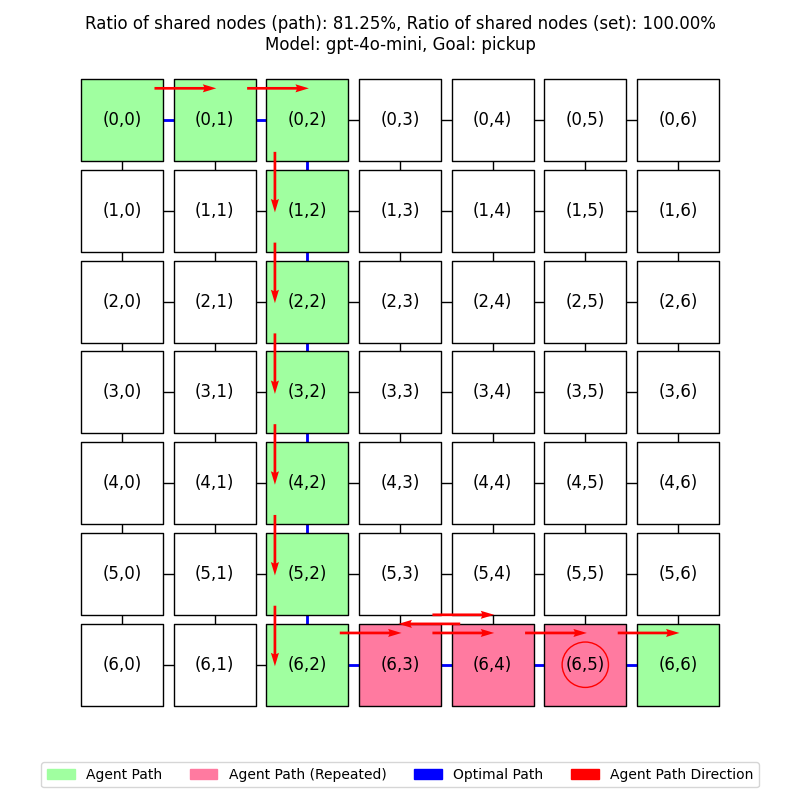
\includegraphics[width=0.5\textwidth]{
    images/results_discussion/stateful/pickupBR_7x7.png
  }
  \caption{Path visualization for stateful agent with pickup goal in the bottom
  right cell}
  \label{fig:stateful_path}
\end{figure}

A dedicated visualization script has been developed to illustrate the agent's
path on the map. This script identifies all optimal paths connecting the start and
the goal, selects the one sharing the highest number of common cells with the
agent's path, and then calculates both the percentage of overlapping cells and the
relative difference in path length. Figure \ref{fig:stateful_path} displays an
example output, highlighting that although the agent eventually reaches the goal,
it encounters difficulties navigating in the vicinity of the goal, as discussed in
Section \ref{sub:pickup_goal_at_the_center}.

\section{``Path Finding''}

Up to this point, we have observed that, in almost every instance, the KnowNo framework
consistently discarded actions related to the agent's goals, such as picking up
and delivering parcels. To determine whether these goal-related actions still contributed
significantly to the agent's uncertainty, we designed an experiment where the
objective was reduced to simply reaching a specific tile.

To implement this, we removed the pickup and delivery actions from the prompt while
keeping all other conditions unchanged. The goal was set up as just reaching a
specific tile, similarly to what the ``Pickup goal'' requires. By doing so, we aimed
to isolate and examine the role of these actions in influencing the agent's uncertainty.
The results of this experiment are presented in Figure \ref{fig:path_finding}. This
approach aligns with our systematic methodology, as previously discussed in
Section \ref{sec:closest_cell_to_the_goal}, where we progressively simplified the
agent's goals to identify potential limitations in decision-making.

A meaningful comparison can be drawn between these results and those obtained from
a scenario in which the agent operated on a 5x5 grid with a pickup goal located at
the center. Since both setups shared the same prompt structure, this comparison allows
us to assess whether the presence of goal-related actions had a significant impact
on the agent's uncertainty. The results from the 5x5 pickup scenario, previously
discussed, can be found in Figure \ref{fig:hm_5x5_pickup} and Figure
\ref{fig:chm_5x5_pickup}.

\begin{figure}[h!]
  \centering
  \begin{minipage}[b]{0.45\textwidth}
    \centering
    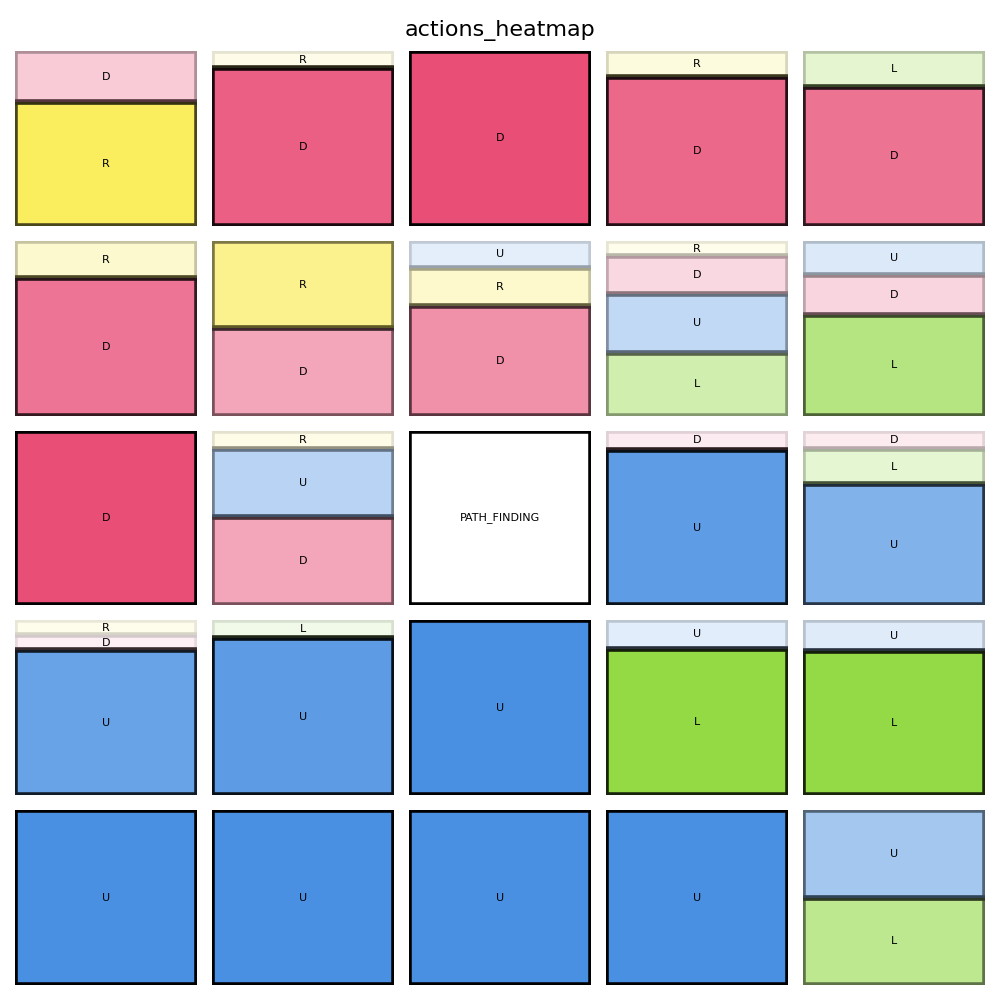
\includegraphics[width=\textwidth]{
      images/results_discussion/path_finding/actions_heatmap.png
    }
    \caption{Heatmap for pathfinding }
    \label{fig:path_finding_hm}
  \end{minipage}
  \hfill
  \begin{minipage}[b]{0.45\textwidth}
    \centering
    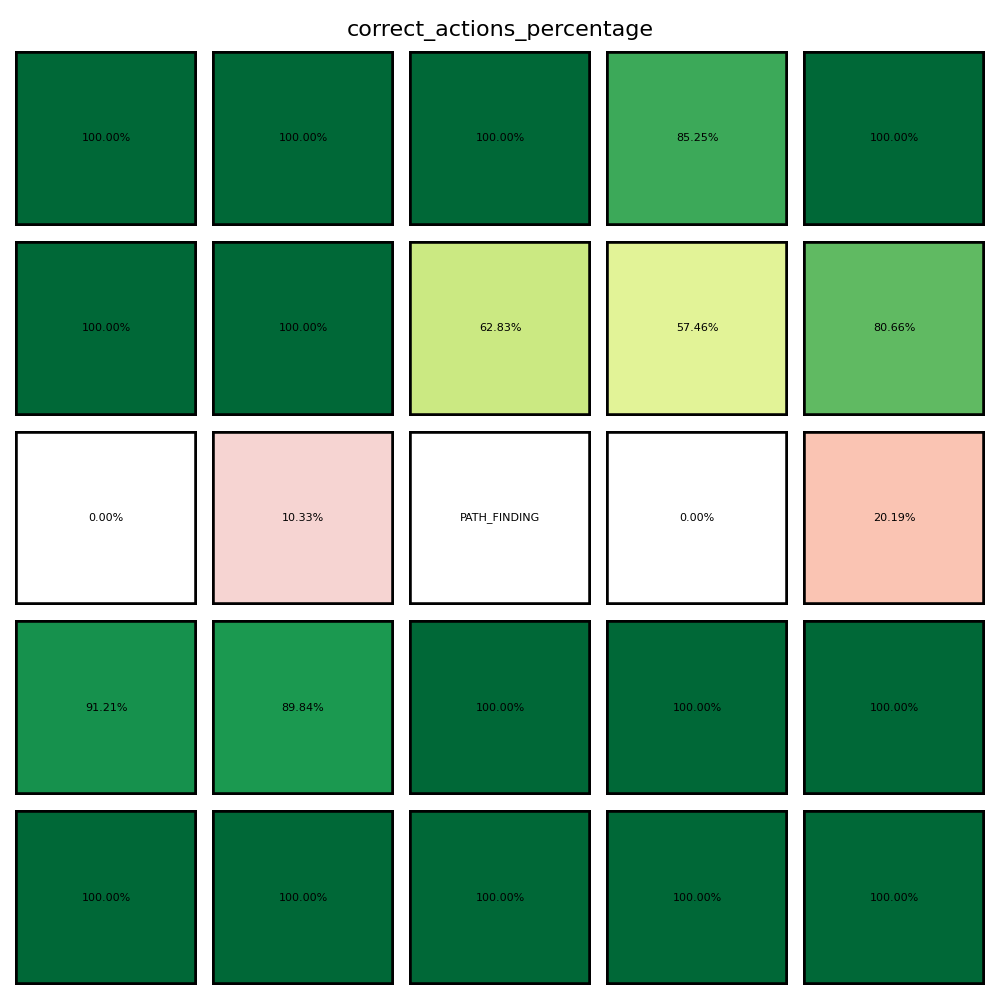
\includegraphics[width=\textwidth]{
      images/results_discussion/path_finding/correct_actions_percentage_PERC.png
    }
    \caption{Correctness for pathfinding}
    \label{fig:path_finding_corr}
  \end{minipage}
  \caption{Heatmaps for stateless agent with pathfinding goal}
  \label{fig:path_finding}
\end{figure}

The outcomes of both experiments are remarkably similar, revealing identical
areas of high and low uncertainty. This suggests that goal-related actions are not
the primary source of uncertainty in the agent's decision-making process.
Furthermore, it reinforces the idea that the structure of the prompt, carefully
designed based on the literature reviewed as explained in Section
\ref{sec:prompt_creation_choices}, is not a key factor contributing to uncertainty.
Instead, the observed uncertainty may be more closely linked to the inherent limitations
of the LLM itself.

\section{Stateless \& Stateful - Performance Summary}
\label{sec:stateless_and_stateful_combined_results}

Experimental results in this study indicate that the stateful configuration
outperforms the stateless one in terms of accuracy and goal attainment, particularly
in larger maps. The ability to trace its previous actions and incorporate
historical context leads to a more adaptive and flexible approach, which is evident
in tasks requiring dynamic path corrections and strategic foresight. During the
first stages of the experiments, where we tried the limits of the token input size,
the stateless agent was not able at all to achieve any goal in maps bigger than
21x21, while the stateful agent was on the correct path but blocked by the token
limit. This is a clear demonstration of the stateful agent's superior
performance in handling complex spatial navigation tasks.

Additionally, the stateful method aligns well with the inherent strengths of large
language models as few-shot learners \cite{brown2020languagemodelsfewshotlearners}.
The continuous integration of historical data and real-time inputs allows the
agent to refine its internal representation of the map, which significantly improves
its overall navigational performance. This dynamic adjustment provides
resilience against uncertainties common in spatial navigation tasks.

Practically speaking, the stateful agent demonstrates a clear advantage in navigating
the "problematic" areas of the maps, particularly in the top-right quadrant, where
the stateless version exhibits significant uncertainty. This improvement arises
from the stateful agent's ability to retain memory of its past actions, enabling
it to recognize and correct mistakes. If it takes a step in the wrong direction,
it can backtrack to a previous cell and attempt an alternative route, ultimately
increasing its chances of reaching the goal efficiently.

However, as the map size increases, both versions encounter growing difficulties,
with the top-right quadrant consistently presenting the most challenges. This
issue stems from the nature of decision-making in that region: many cells offer multiple
actions with nearly equal probabilities, making it harder for the agent to
determine the optimal path. While the relative frequency of these problematic cells
remains constant as the map scales up, the absolute number of such cells
increases substantially. For example, in a small 3x3 map, a single problematic cell
is manageable, as the agent can quickly backtrack and reach the goal. In contrast,
in a much larger 21x21 map, there could be as many as 49 problematic cells. Even
though this proportion is the same in percentage terms, the larger map exacerbates
the challenge. With more problematic cells spread across a wider area, the agent
is more likely to make a series of unfortunate steps, potentially getting
trapped in a suboptimal loop and failing to recover efficiently. This issue is particularly
severe for the stateless agent, but even the stateful agent, despite its ability
to backtrack, can struggle to escape if the problematic region is too large.

A summary of their performance are presented in the table \ref{tab:svss}, where the
agent was tasked to pickup a parcel in the bottom left cell and started in the top
right cell (since it is the most problematic area). The recorded action count
includes the pickup action.

\vspace{5mm}
\begin{table}[h]
  \centering
  \begin{tabular}{c|cc|c}
    \textbf{Map Size} & \textbf{Stateless} & \textbf{Stateful} & \textbf{Mathematical Best} \\
    \hline
    13x13             & 41 actions         & 39 actions        & 25 actions                 \\
    7x7               & 27 actions         & 21 actions        & 13 actions                 \\
    5x5               & 14 actions         & 11 actions        & 9 actions                  \\
    3x3               & 11 actions         & 9 actions         & 5 actions                  \\
  \end{tabular}
  \caption{Number of actions in different map sizes using GPT-4o-mini}
  \label{tab:svss}
\end{table}
\vspace{5mm}

In summary, although the stateful approach can introduce computational overhead
due to increased context size, its advantages in enhancing navigational accuracy,
recovery from errors, and adaptive decision-making render it a vital component in
modern agent design. Still, the limitation of the token limit is a significant drawback
that may be overcome by more powerful models, that may introduce better results
out of the box as well as a longer context window.

\section{Insights from the Closest Cell to the Goal Approach}
\label{sec:closest_cell_to_the_goal_results}

As detailed in Section \ref{sec:closest_cell_to_the_goal}, this approach aimed
to simplify the agent's decision-making process by breaking it down into two
sequential steps: (1) identifying the best adjacent cell to move toward and (2) selecting
the correct action to reach that cell. The motivation behind this decomposition
was to reduce the complexity of the global path-finding task and test whether
the agent could make more reliable local decisions.

Although this method was not central to our primary experiments, we include it here
for completeness, as analyzing its shortcomings provided useful insights into
the agent's limitations.

Despite its structured nature, this method introduced new challenges rather than
resolving the agent's decision-making issues. In particular, two key limitations
emerged:
\begin{itemize}
  \item Ambiguity in selecting the ``best" cell: In many cases, more than one
    neighboring cell reduced the distance to the goal, making it unclear which one
    the agent should prioritize and more difficult to us to record structured data
    to analyze. As illustrated in Figure \ref{fig:extra2}, the decision was not always
    straightforward, and slight variations in prompt phrasing could lead the LLM
    to prefer different paths, even when multiple valid choices existed;

  \item Compounding errors in high-uncertainty areas: This two-step approach
    inadvertently introduced an additional layer of failure. If the agent misidentified
    the best neighboring cell, it would inherently lead to a suboptimal move, even
    if the second step—choosing the action—was executed perfectly. This doubled
    the impact of errors, particularly in ambiguous or low-information regions of
    the map, where uncertainty was already high.
\end{itemize}

\vspace{7mm}
\begin{figure}[h!]
  \centering
  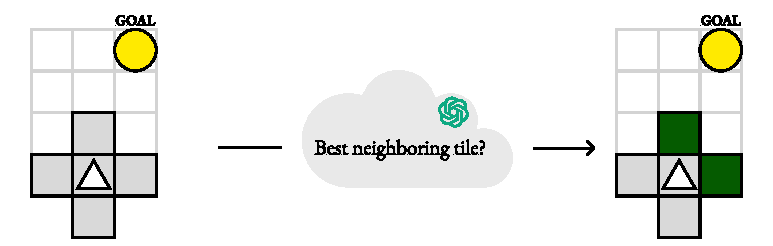
\includegraphics[width=.66\textwidth]{images/results_discussion/extra2.pdf}
  \caption{Two-steps decision making problem}
  \label{fig:extra2}
\end{figure}
\vspace{7mm}

\section{Model Comparison}
\label{sec:model_comparison}

As mentioned in previous sections, our experiments primarily utilized GPT-4o-mini,
a smaller variant of the GPT-4o model. This choice was mainly influenced by cost
considerations and its performance relative to the full GPT-4o model. We also evaluated
GPT-3.5-turbo, an older model, and found that while its overall capabilities were
not necessarily worse, it was less likely to select the correct action as the
one with the highest probability compared to GPT-4o-mini.

\begin{figure}[h]
  \centering
  \begin{minipage}[b]{0.32\textwidth}
    \centering
    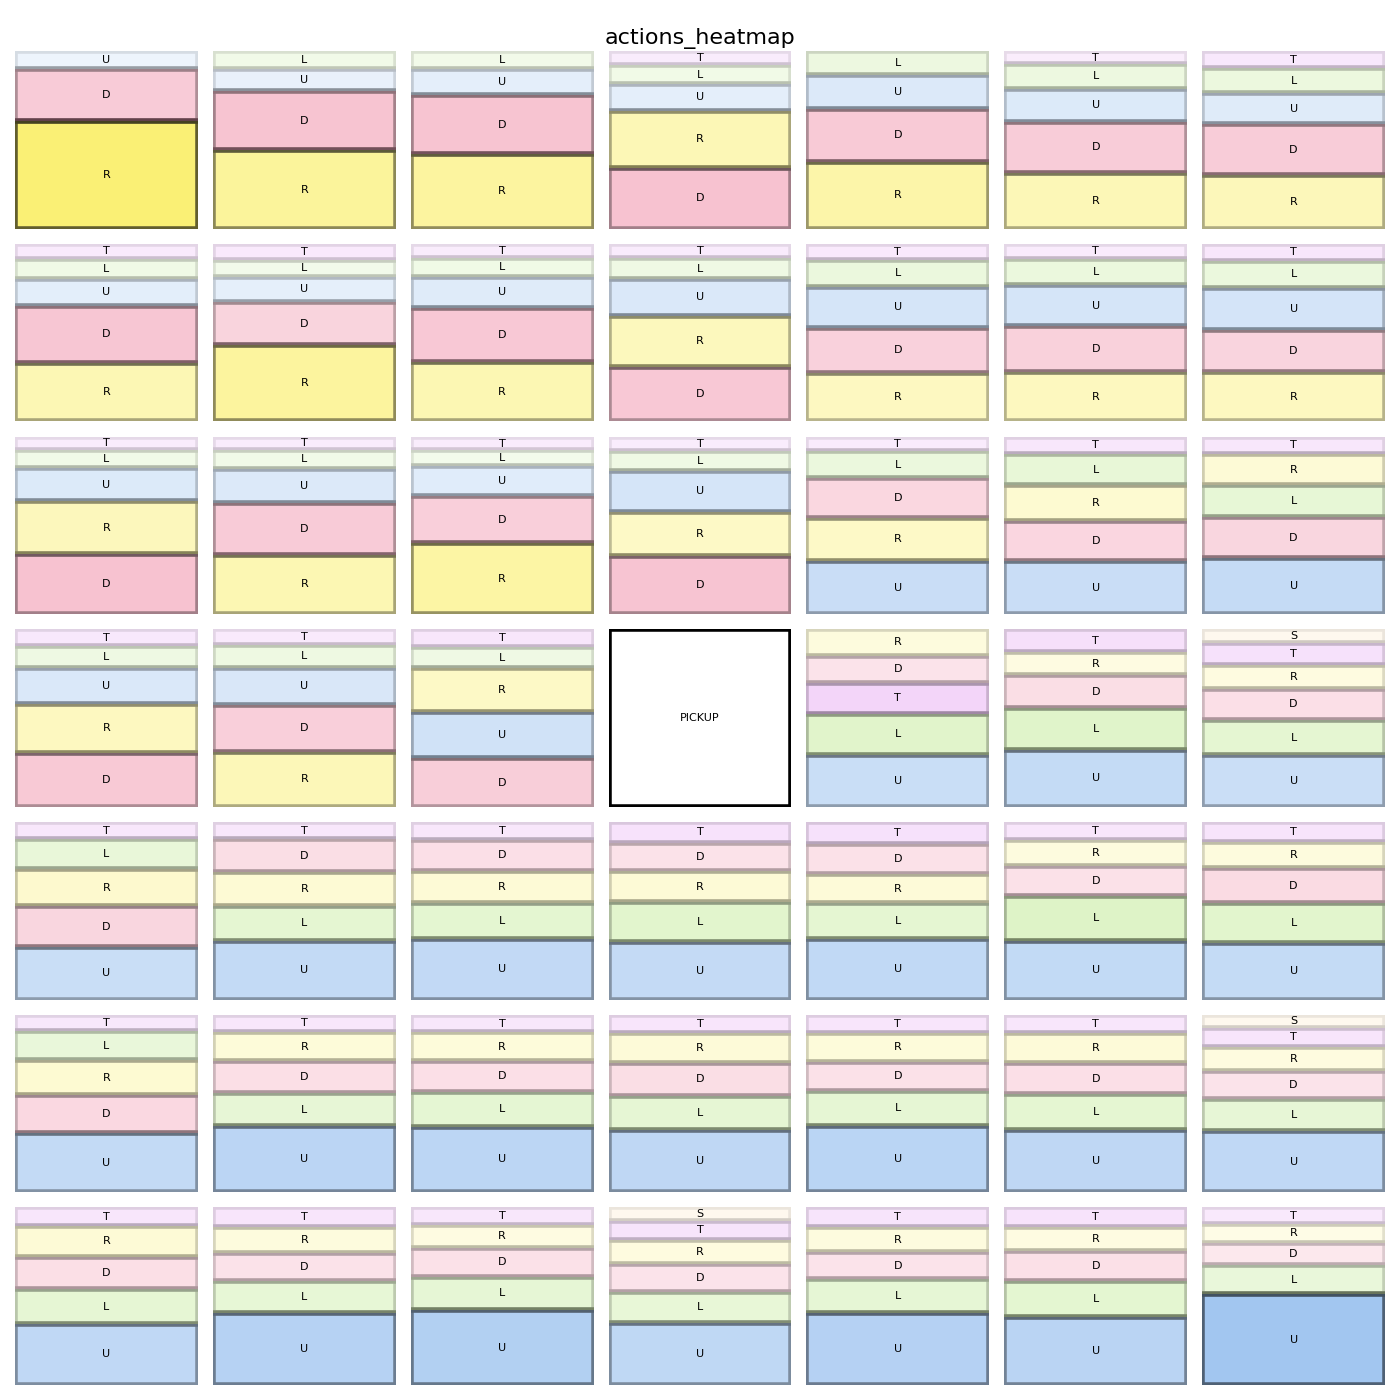
\includegraphics[width=\textwidth]{
      images/results_discussion/models/GPT3.5-turbo/actions_heatmap.png
    }
    \caption{GPT-3.5-turbo}
    \label{fig:models_gpt35}
  \end{minipage}
  \hfill
  \begin{minipage}[b]{0.32\textwidth}
    \centering
    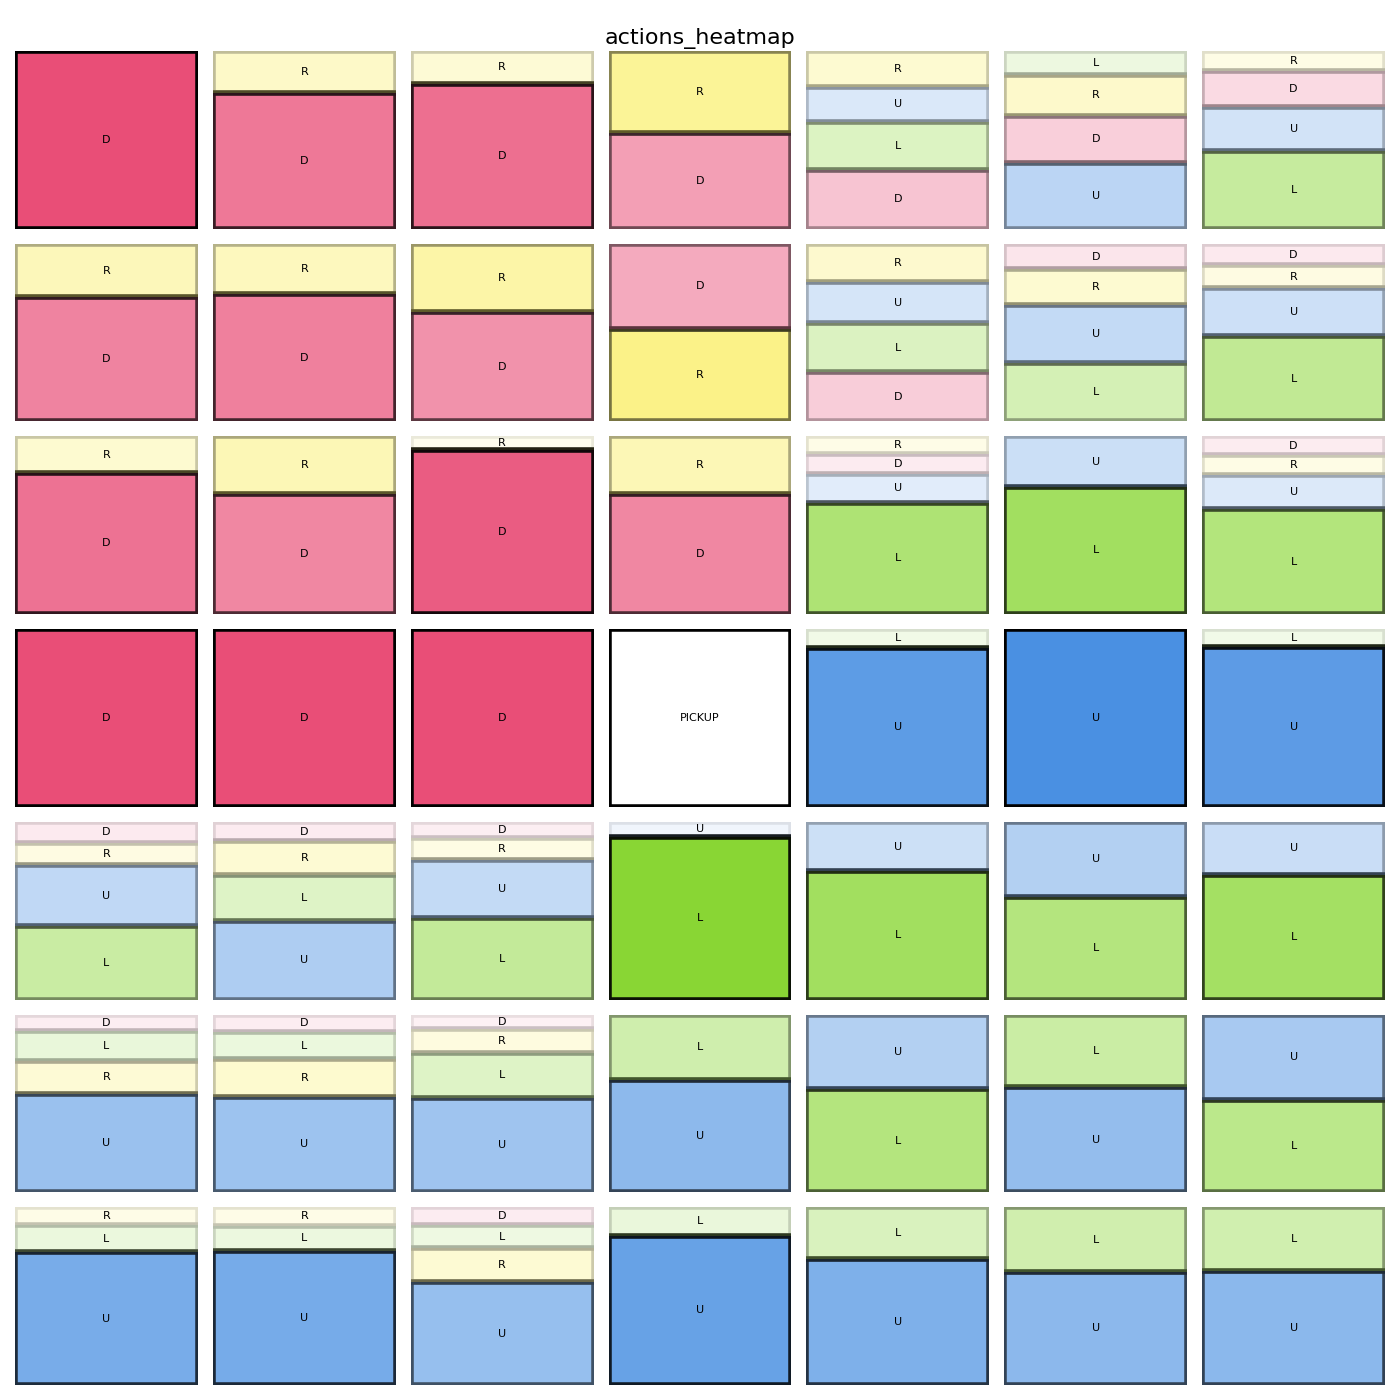
\includegraphics[width=\textwidth]{
      images/results_discussion/models/GPT4o/actions_heatmap.png
    }
    \caption{GPT-4o}
    \label{fig:models_gpt4o}
  \end{minipage}
  \hfill
  \begin{minipage}[b]{0.32\textwidth}
    \centering
    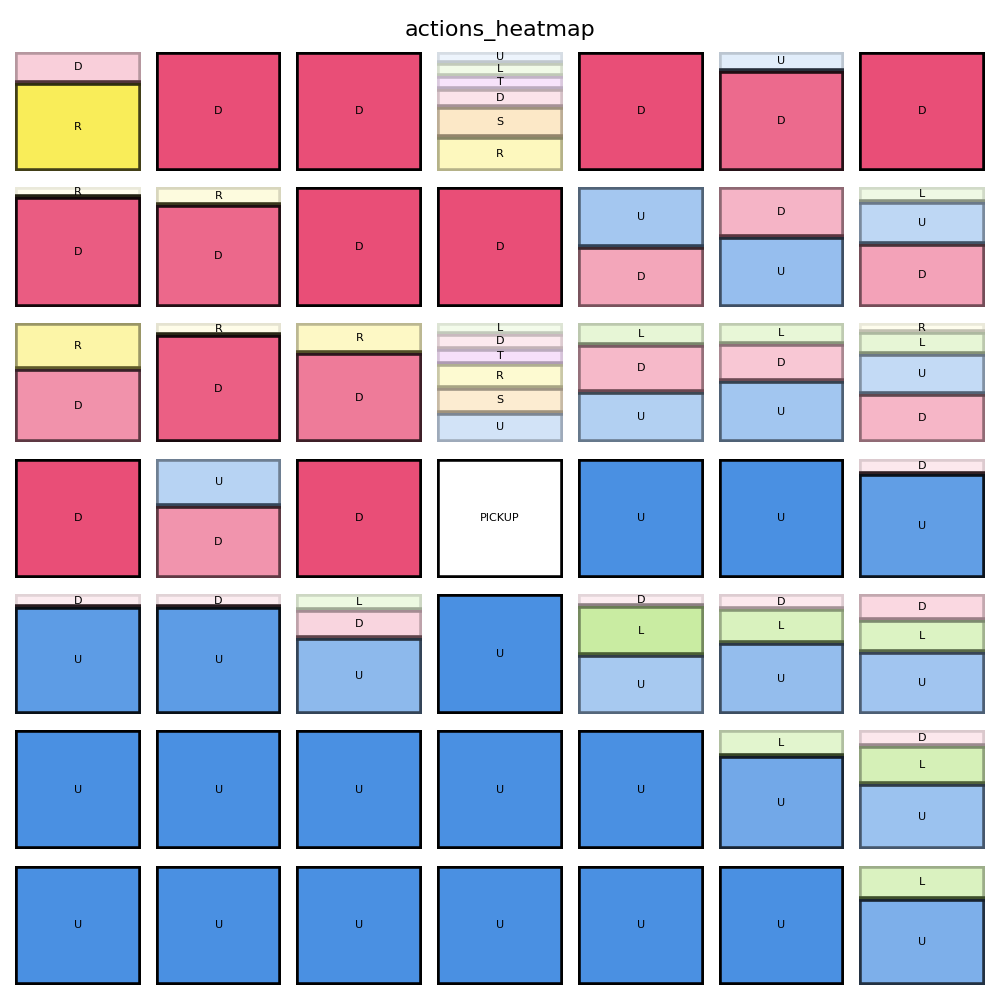
\includegraphics[width=\textwidth]{
      images/results_discussion/models/GPT4o-mini/actions_heatmap.png
    }
    \caption{GPT-4o-mini}
    \label{fig:models_gpt4o_mini}
  \end{minipage}
  \caption{Heatmaps for different GPT models}
  \label{fig:models_hm}
\end{figure}

Results obtained with GPT-4o-mini closely align with those of GPT-4o, ensuring
that all discussions in this document remain applicable to both models. From Table
\ref{tab:model_comparison}, we can see that GPT-3.5-turbo selects the correct
action as the highest probability option less frequently than the other models, though
its top-2 and top-3 probabilities remain comparable.

\vspace{5mm}
\begin{table}[h]
  \centering
  \begin{tabular}{c|ccc|ccc}
    \hline
                  & top1 & top2 & top3 & top1\% & top2\% & top3\% \\
    \hline
    GPT-3.5-turbo & 34   & 46   & 48   & 0.708  & 0.958  & 1.000  \\
    GPT-4o        & 37   & 44   & 44   & 0.771  & 0.917  & 0.917  \\
    GPT-4o-mini   & 37   & 40   & 41   & 0.771  & 0.833  & 0.854  \\
    \hline
  \end{tabular}
  \caption{Comparison between different GPT models in a 7x7 map}
  \label{tab:model_comparison}
\end{table}
\vspace{5mm}

However, Figures \ref{fig:models_hm} and \ref{fig:models_chm} clearly show that GPT-3.5-turbo
exhibits greater overall uncertainty. Still, this demonstrates that our experimental
setup is adaptable to different models and effectively structured to assess the capabilities
of LLMs in this task.

\begin{figure}[h]
  \centering
  \begin{minipage}[b]{0.32\textwidth}
    \centering
    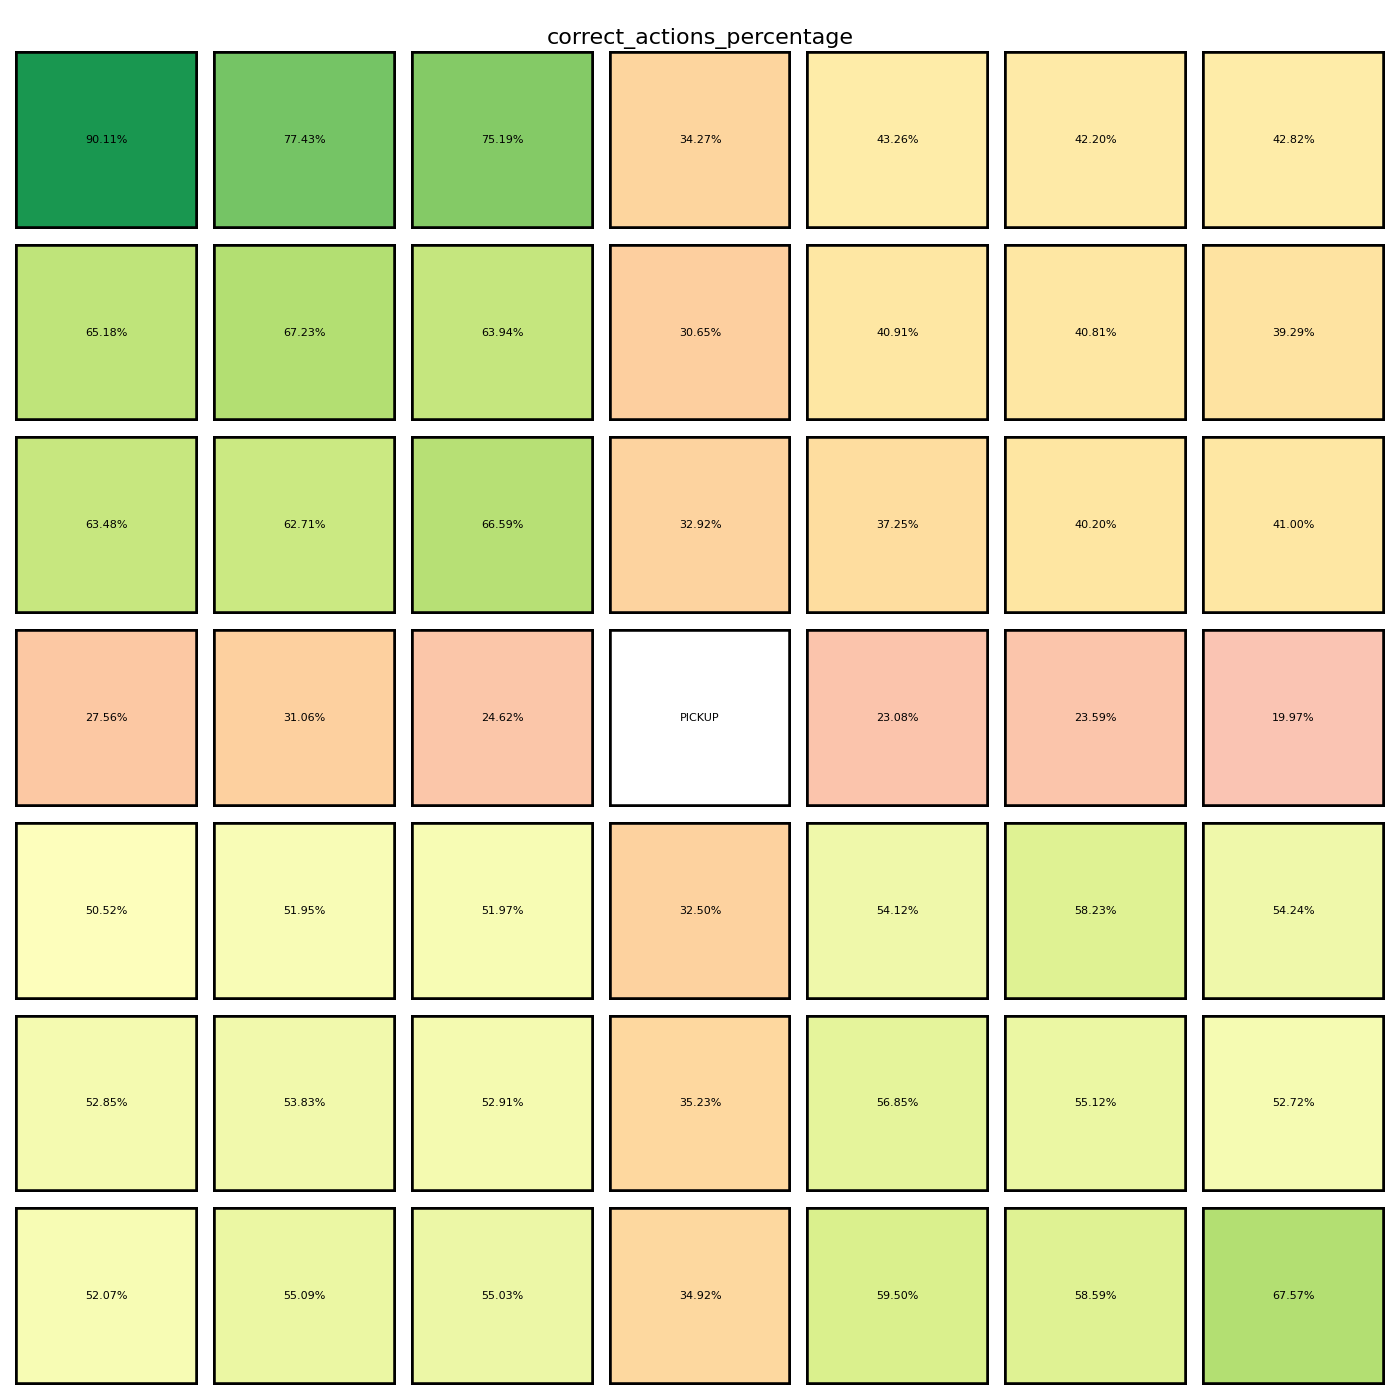
\includegraphics[width=\textwidth]{
      images/results_discussion/models/GPT3.5-turbo/correct_actions_percentage_PERC.png
    }
    \caption{GPT-3.5-turbo}
    \label{fig:models_gpt35}
  \end{minipage}
  \hfill
  \begin{minipage}[b]{0.32\textwidth}
    \centering
    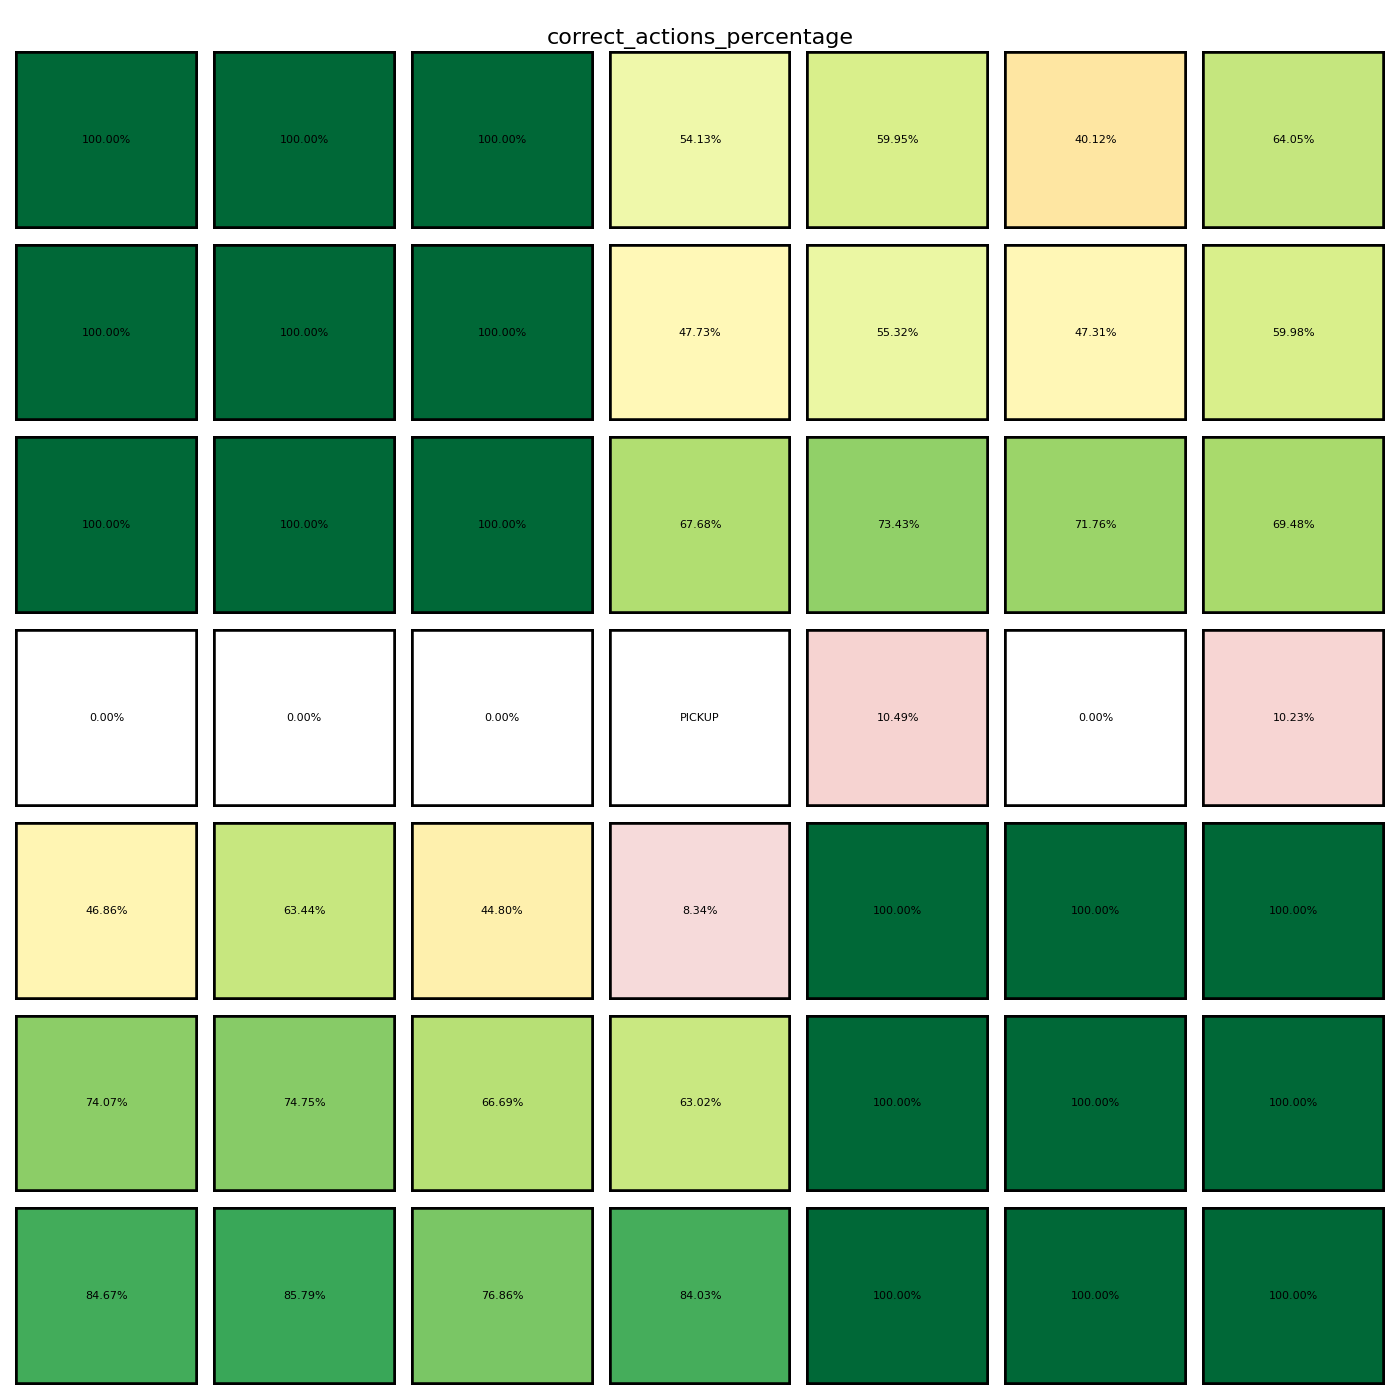
\includegraphics[width=\textwidth]{
      images/results_discussion/models/GPT4o/correct_actions_percentage_PERC.png
    }
    \caption{GPT-4o}
    \label{fig:models_gpt4o}
  \end{minipage}
  \hfill
  \begin{minipage}[b]{0.32\textwidth}
    \centering
    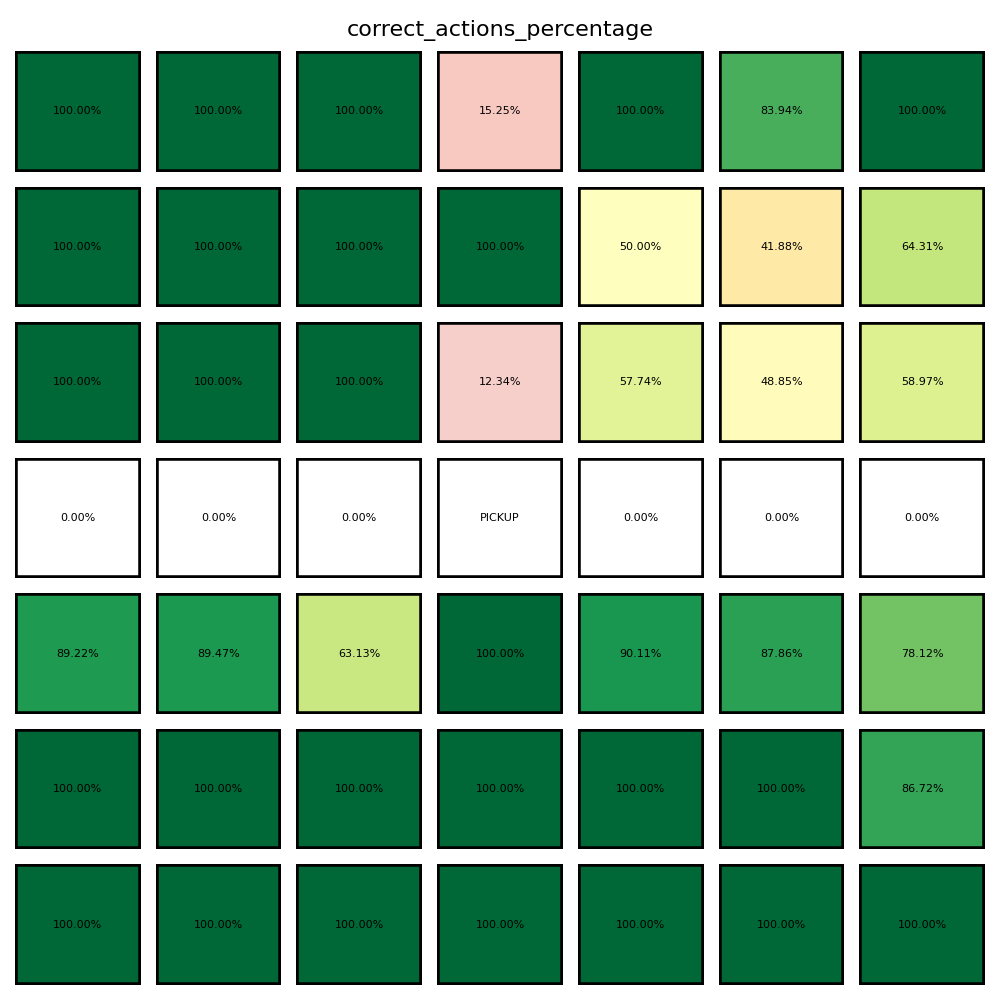
\includegraphics[width=\textwidth]{
      images/results_discussion/models/GPT4o-mini/correct_actions_percentage_PERC.png
    }
    \caption{GPT-4o-mini}
    \label{fig:models_gpt4o_mini}
  \end{minipage}
  \caption{Correctness Heatmaps for different GPT models}
  \label{fig:models_chm}
\end{figure}